\documentclass[a4paper,11pt]{article}
\usepackage[utf8]{inputenc}
\usepackage{graphicx}
\usepackage{amsmath,amssymb}
\usepackage{booktabs}
\usepackage{longtable}
\usepackage{hyperref}
\usepackage{geometry}
\usepackage{array}
\usepackage{seqsplit}
\geometry{margin=1in}
\graphicspath{{figures/}}
\setlength{\emergencystretch}{2em}
\renewcommand{\thefigure}{S\arabic{figure}}
\renewcommand{\thetable}{S\arabic{table}}

\title{\textbf{Supplementary Material}\\[6pt]
Spatio-temporal wall-actuation modes and cycle-mean\\
viscous dissipation in a lid-driven cavity}

\author{Beniaiche Ahmed\(^{1}\), Larabi Abderrahim\(^{1}\), Belkadi Mbarek\(^{2}\) \\[4pt]
\(^{1}\)Laboratory of Fluid Mechanics, Ecole Militaire Polytechnique, Algiers, Algeria \\
\(^{2}\)Laboratory of Turbomachinery, Ecole Militaire Polytechnique, Algiers, Algeria}
\date{}

\begin{document}

\maketitle
\tableofcontents
\newpage

%=============================================================
\section*{Overview}
%=============================================================

This Supplementary Material accompanies the manuscript \textit{``Spatio-temporal
wall-actuation modes and cycle-mean viscous dissipation in a lid-driven cavity''}.
It
contains detailed numerical formulations, complete network architecture
specifications, cell- and seed-level campaign datasets for all sensitivity campaigns,
grid-convergence calculations, the wall-shear estimator analysis, and reproducibility
guidelines. The material is organized so that the main text can be read as a
fluid-mechanics paper: every result that concerns the identification procedure, the
variational landscape, the sensitivity campaigns or the numerical verification is
documented here, while the main text retains only the physical formulation, the
actuation modes, the dissipation comparison and its interpretation. All section
numbers in this document are prefixed with ``S'' to distinguish them from main-text
sections, and all figures are numbered S1, S2, \ldots{} independently of the main
text. The tables are numbered in the same way, so that Table~S1 of this document is
distinct from Table~1 of the main text. Cross-references to the main manuscript use
the notation (Main Sec., Main Fig.~X or Main Table~X).

%=============================================================
\section{S1. Detailed PINN Implementation}
%=============================================================

\subsection{S1.1 Network Architecture Specifications}

The physics-informed optimization employs two separate fully connected neural
networks operating in double-precision (float64) arithmetic throughout: a
\emph{flow network} that represents the velocity and pressure fields
\((u,v,p)(x,y,t;\widetilde{Re})\), and a \emph{control network} that represents
the spatio-temporal Fourier coefficients \(a_{mn}(\widetilde{Re})\). The two
networks share the same input normalization but have different widths and depths,
reflecting the different complexity of the flow field and the low-dimensional
control space.

\textbf{Input normalization.} The spatial coordinates \((x,y)\in[0,L_x]\times[0,1]\)
and time \(t\in[0,1]\) are fed directly to the networks. The Reynolds number is
normalized to
\begin{equation}
\widetilde{Re}=\frac{Re-550}{450}\in[-1,1],
\end{equation}
so that the training range \(Re\in[100,1000]\) maps to \([-1,1]\), improving
numerical conditioning of the gradient computations.

\textbf{Flow network.} Six hidden layers, each with 64 neurons, using hyperbolic
tangent (\(\tanh\)) activation functions. Inputs: \((x,y,t,\widetilde{Re})\),
dimension 4. Outputs: \((u,v,p)\), dimension 3. Total trainable parameters:
\(4\times64 + 5\times(64\times64+64) + 64\times3+3 = 21\,379\).

\textbf{Control network.} Four hidden layers, each with 32 neurons, using \(\tanh\)
activation. Inputs: \((\widetilde{Re})\), dimension 1. Outputs:
\(\{a_{mn}\}_{m=1,\ldots,N_x;\,n=0,\ldots,N_t-1}\), dimension \(N_x\times N_t=30\)
(baseline). Total trainable parameters: \(1\times32+4\times(32\times32+32)+32\times30+30=3\,614\).

\textbf{Initialization.} All network weights are initialized using the
Xavier/Glorot normal distribution with zero-mean and variance
\(\sigma^2=2/(n_{\mathrm{in}}+n_{\mathrm{out}})\) where \(n_{\mathrm{in}}\) and
\(n_{\mathrm{out}}\) are the fan-in and fan-out of each layer. All biases are
initialized to zero.

\textbf{Precision.} All weight tensors, input tensors, automatic differentiation
operations, and loss evaluations use 64-bit (double) precision. This choice avoids
numerical cancellation in the evaluation of the PDE residuals, which involve
second-order derivatives of the network outputs.

Table~\ref{tab:s1_network} summarizes the architecture specifications.

\begin{table}[h]
\centering
\caption{Neural network architecture specifications for flow and control networks.}
\label{tab:s1_network}
\small
\begin{tabular}{lccccc}
\toprule
Network & Layers & Neurons & Activation & Inputs & Outputs\\
\midrule
Flow    & 6 hidden + I/O & 64 & \(\tanh\) & 4 & 3 (u,v,p)\\
Control & 4 hidden + I/O & 32 & \(\tanh\) & 1 & 30 (\(a_{mn}\))\\
\bottomrule
\end{tabular}
\end{table}

\subsection{S1.2 Collocation Sampling and Initialization}

All collocation points are resampled from scratch at the beginning of each
training epoch, preventing overfitting to any fixed quadrature set.

\textbf{Interior PDE collocation:} \(N_{\mathrm{phys}}=4\,000\) points sampled
uniformly at random over the computational domain
\(\Omega\times[0,1]=[0,L_x]\times[0,1]\times[0,1]\). At each epoch, three
Reynolds-number values are selected from the set \(\{100,300,500,700,900,1000\}\);
each interior point is evaluated at all three selected \(Re\) values, giving an
effective PDE sample size of \(3N_{\mathrm{phys}}=12\,000\) residual evaluations
per epoch.

\textbf{Boundary collocation:} \(N_{\mathrm{BC}}=600\) points distributed across
the boundary \(\partial\Omega\), split as \(200\) on \(\Gamma_{\mathrm{top}}\)
(upper lid) and \(400\) on \(\Gamma_{\mathrm{stat}}\) (bottom and lateral walls),
resampled uniformly at each epoch.

\textbf{Reynolds parameter:} During each epoch, 6 discrete Reynolds values
($100$, $300$, $500$, $700$, $900$, $1000$) are used for boundary-condition
enforcement and the Reynolds-separation regularization.

\subsection{S1.3 Optimization Schedule and Hyperparameters}

Training proceeds in two stages:

\textbf{Stage 1 --- Pre-training (300 epochs):} Only the flow network weights
are updated. The control coefficients \(a_{mn}\) are frozen at zero, preventing
the optimizer from immediately collapsing to degenerate control solutions before
a physically consistent flow representation has been established. During this
stage, only the PDE residual, boundary-condition, and Reynolds-separation losses
are active (the dissipation and energy objectives depend on flow accuracy to be
meaningful).

\textbf{Stage 2 --- Joint optimization (3\,000 epochs):} All flow and control
network weights are updated simultaneously. The full multi-objective loss
(Main Eq.~(13)) is active with the reference weights listed after that equation.

\textbf{Optimizer:} Adam with \(\beta_1=0.9\), \(\beta_2=0.999\),
\(\epsilon_{\mathrm{Adam}}=10^{-8}\).

\textbf{Learning rate schedule:} Initial rate \(\eta_0=8\times10^{-4}\) with
exponential decay by factor \(0.995\) every 100 epochs, giving
\(\eta(e)=\eta_0\times0.995^{\lfloor e/100\rfloor}\). After 3\,000 epochs, the
effective learning rate is approximately \(8\times10^{-4}\times0.995^{30}
\approx 6.9\times10^{-4}\), so the learning rate has decayed by only \(\sim14\%\)
over the full training. No gradient clipping is applied.

\textbf{Convergence behavior:} Typical behavior over the 3\,000-epoch joint phase
shows \(\mathcal{L}_{\mathrm{PDE}}\) reaching approximately \(10^{-3}\) by epoch
3\,000, \(\mathcal{L}_{\mathrm{BC}}\) below \(5\times10^{-4}\), and
\(\mathcal{L}_{\mathrm{ctrl}}\) below \(10^{-4}\) (corresponding to
\(|E_r-E^*|<10^{-2}\)). The total loss value at convergence lies in the range
\([1.37,1.40]\) for the \((Re,E^*)=(500,0.25)\) condition used in the seed study.

\textbf{Seed sensitivity:} The early training stochasticity during Stage 1
determines which outcome cluster is entered during Stage 2. Once Stage 2 begins,
the optimizer rarely switches clusters, explaining the reproducible classification
of each realization. No early stopping is applied; all realizations run for the full
3\,000 epochs regardless of convergence.

\subsection{S1.4 Multi-Objective Loss Formulation}

The complete loss is (Main Eq.~(13)):
\begin{equation}
\mathcal{L}=\lambda_{\mathrm{PDE}}\mathcal{L}_{\mathrm{PDE}}
+\lambda_{\mathrm{BC}}\mathcal{L}_{\mathrm{BC}}
+\lambda_{\mathrm{diss}}\mathcal{L}_{\mathrm{diss}}
+\lambda_{\mathrm{ctrl}}\mathcal{L}_{\mathrm{ctrl}}
+\lambda_{\mathrm{var}}\mathcal{L}_{\mathrm{var}}
+\lambda_{Re}\mathcal{L}_{Re},
\end{equation}
with baseline weights \(\lambda_{\mathrm{PDE}}=1\), \(\lambda_{\mathrm{BC}}=15\),
\(\lambda_{\mathrm{diss}}=0.05\), \(\lambda_{\mathrm{ctrl}}=200\),
\(\lambda_{\mathrm{var}}=1\), \(\lambda_{Re}=2\). The individual components are:
\begin{align}
\mathcal{L}_{\mathrm{PDE}}&=\left\langle R_u^2+R_v^2+R_c^2\right\rangle_{\mathcal{X}_{\mathrm{int}}},\\
\mathcal{L}_{\mathrm{BC}}&=\left\langle u^2+v^2\right\rangle_{\Gamma_{\mathrm{stat}}}
+\left\langle(u-U_{\mathrm{lid}})^2+v^2\right\rangle_{\Gamma_{\mathrm{top}}},\\
\mathcal{L}_{\mathrm{diss}}&=\int_\Omega\frac{1}{Re}
\!\left[u_x^2+v_y^2+\tfrac{1}{2}(u_y+v_x)^2\right]d\Omega
=\int_\Omega\nu\,S{:}S\,d\Omega,\\
\mathcal{L}_{\mathrm{ctrl}}&=(E_r-E^*)^2,\\
\mathcal{L}_{\mathrm{var}}&=-\log\!\left[\operatorname{Var}(U_{\mathrm{lid}})+10^{-5}\right],\\
\mathcal{L}_{Re}&=\max\!\left[0,\;\delta-
\frac{1}{N_{\mathrm{probe}}}\sum_{i=1}^{N_{\mathrm{probe}}}
\!\left(U_{\mathrm{lid}}(x_i,t_0,Re_{\min})
-U_{\mathrm{lid}}(x_i,t_0,Re_{\max})\right)^2\right],
\end{align}
with \(N_{\mathrm{probe}}=20\) probe locations distributed uniformly in \(x\in[0,L_x]\),
\(t_0=0.5\), \(\delta=0.01\), \(Re_{\min}=100\), \(Re_{\max}=1000\).

No initial-condition term is included by design. The temporal Fourier expansion
and the cycle-averaged objective define a periodic space--time boundary-value
problem, so training targets a statistically stationary periodic state rather
than the transient from a prescribed initial field (Main Sec.~4.1).

\textbf{Weight rationale.} The weight \(\lambda_{\mathrm{BC}}=15\) strongly
enforces boundary conditions relative to the interior residual, preventing poorly
conditioned flow states where boundary violations dominate the solution.
\(\lambda_{\mathrm{ctrl}}=200\) is large to enforce the energy constraint tightly
(\(|E_r-E^*|/E^*<5\%\) at convergence for all tested conditions), ensuring that
all realizations are compared at effectively the same actuation energy. The small
value \(\lambda_{\mathrm{diss}}=0.05\) prevents the dissipation objective from
overwhelming the PDE constraints during early training, which can cause the
optimizer to ignore physical accuracy in favor of reducing dissipation. The
regularizer \(10^{-5}\) in \(\mathcal{L}_{\mathrm{var}}\) prevents numerical
issues when \(\operatorname{Var}(U_{\mathrm{lid}})=0\) at the beginning of training
before the control network has been activated.

%=============================================================
\section{S2. Control-Space and Modal-Analysis Details}
%=============================================================

\subsection{S2.1 Spatio-Temporal Fourier Basis}

The boundary actuation is expanded as in Main Sec.~3.2:
\begin{equation}
U_{\mathrm{lid}}(x,t,Re)=\sum_{m=1}^{N_x}\sum_{n=0}^{N_t-1}
a_{mn}(Re)\sin\!\left(\frac{m\pi x}{L_x}\right)\cos(n\pi t),
\end{equation}
with baseline truncation \(N_x=6\), \(N_t=5\), giving 30 nominal coefficients.
The sine basis \(\sin(m\pi x/L_x)\) is chosen because it vanishes at
\(x=0\) and \(x=L_x\) for all \(m\ge1\), automatically enforcing corner
compatibility without any additional constraint. The cosine basis \(\cos(n\pi t)\)
has the property that \(\cos(0\cdot\pi t)=1\), so the \(n=0\) terms represent
purely stationary (time-independent) actuation. All mode indices in this manuscript
use the physical (one-based) convention: the second spatial harmonic corresponds
to \(m=2\), not \(m=1\).

\subsection{S2.2 Modal Energy Normalization and Quadrature}

The time-average of the squared basis functions satisfies
\(\langle\cos^2(0)\rangle_t=1\) and \(\langle\cos^2(n\pi t)\rangle_t=\frac{1}{2}\)
for \(n\ge1\). The space-average of the squared sine basis functions satisfies
\(\langle\sin^2(m\pi s)\rangle_s=\frac{1}{2}\) for all \(m\ge1\),
where \(s=x/L_x\in[0,1]\). Therefore, the contribution of coefficient \(a_{mn}\)
to the realized energy \(E_r=\langle U_{\mathrm{lid}}^2\rangle_{s,t}\) is:
\begin{equation}
E_{mn}=\langle a_{mn}^2\sin^2(m\pi s)\cos^2(n\pi t)\rangle_{s,t}
=\begin{cases}
\tfrac{1}{2}a_{m0}^2 & n=0,\\
\tfrac{1}{4}a_{mn}^2 & n\ge1.
\end{cases}
\end{equation}
These are the modal energies \(\mathcal{E}_{mn}\) used in Main Sec.~3.2.
The realized actuation energy is therefore
\begin{equation}
E_r=\sum_{m=1}^{N_x}\left(\tfrac{1}{2}a_{m0}^2
+\sum_{n=1}^{N_t-1}\tfrac{1}{4}a_{mn}^2\right).
\end{equation}

\subsection{S2.3 Branch Classification Thresholds}

The branch clusters are defined by the following explicit rule applied in order
to the normalized modal fractions \(f_1\equiv f_{10}\) (stationary first spatial
harmonic), \(f_2\equiv f_{20}\) and
\(f_t=\sum_{m,n\ge1}f_{mn}\):
\begin{itemize}
\item \(B_{\mathrm{first}}\): \(f_1>0.5\) (stationary first harmonic carries an
absolute majority of the actuation energy).
\item \(B_1\): \(f_2>2f_t\) and \(f_2>0.5\) (stationary second mode carries at
least twice the energy of all temporal modes, and more than half of the total).
\item \(B_2\): \(f_t>2f_2\) and \(f_t>0.5\) (temporal family dominant).
\item \(B_3\): none of the above (residual class).
\end{itemize}
This is a dominance rule rather than an absolute cut-off on \(f_2\) or \(f_t\):
a realization is assigned to the class that carries the control energy, and the
rule reproduces the three well-separated groups visible in the
\((f_2,f_t)\) observable space of the identification campaign. The parameters \(k=2\) (dominance
factor) and \(\phi=0.5\) (floor) were fixed a priori and not tuned to the data.

The \(B_{\mathrm{first}}\) test was added after a full-spectrum audit of all 185
realizations and of the \(\lambda_{\mathrm{var}}\) campaign, because the earlier
three-class rule assigned a first-harmonic-dominated control to \(B_3\) whenever
it satisfied neither \(f_2>0.5\) nor \(f_t>0.5\). The audit shows that this defect
never materializes in the broad campaign: \(f_1\le0.122\) over all 185 runs
(\(f_1\le0.096\) within \(B_3\)), so \(B_{\mathrm{first}}\) is empty there and all
185 labels, frequencies and confidence intervals are unchanged
(the class audit of Sec.~S2.3). It does materialize in the ablation campaign,
where removing \(\mathcal{L}_{\mathrm{var}}\) produces \(f_1=0.87\)--\(0.99\)
(Table~\ref{tab:bfirst_ablation}). The audit also resolves what \(B_3\) contains:
15 of its 26 members are dominated by the temporal family, 8 by the stationary
second harmonic and 3 by stationary harmonics of order \(m\ge3\); none by the
first harmonic (sub-structure analysis of Sec.~S2.3).

Table~\ref{tab:s3_threshold} reports the sensitivity of the pooled frequencies
to both \(k\) and \(\phi\): varying \(k\) between \(1.5\) and \(3\), or \(\phi\)
between \(0.4\) and \(0.6\), moves \(\widehat P(B_1)\) and \(\widehat P(B_2)\) by
less than three percentage points and changes at most \(12\) of the \(185\)
realizations. The frequency of the residual class \(B_3\) is more sensitive
(\(9.2\%\)--\(20.5\%\)) because it is defined as the complement of the other
conditions and is the smallest class; its share should therefore be read as
approximate, whereas the \(B_1/B_2\) balance used in this study is robust.
Lowering the \(B_{\mathrm{first}}\) threshold from \(0.5\) to \(0.2\) or even
\(0.13\) would still leave the class empty in this campaign, so the pooled
frequencies are insensitive to that choice. Only \(6\)
realizations lie within \(0.05\) of a dominance boundary, and the smallest
distance to a boundary over the whole campaign is \(0.008\).

% Table P3.5: sensitivity of the branch classification rule
% (auto-generated by scripts/export_legacy_supp_tables.py from
% results/01_ReE_star_map/branch_runs.csv -- do not edit)
\begin{table}[h]
\centering
\caption{Sensitivity of the pooled branch frequencies to the parameters of the dominance rule ($B_1$: $f_2>k f_t$ and $f_2>\phi$; $B_2$: $f_t>k f_2$ and $f_t>\phi$; $B_3$: otherwise). The reference rule is $k=2$, $\phi=0.5$; one parameter is varied at a time. The last column counts the realizations whose label changes with respect to the reference.}
\label{tab:s3_threshold}
\small
\begin{tabular}{lcccccc}
\toprule
Parameter & Value & $B_1$ (\%) & $B_2$ (\%) & $B_3$ (\%) & Reclassified (of 185)\\ 
\midrule
dominance factor $k$ & 1.50 & 43.2 & 47.6 & 9.2 & 9\\
dominance factor $k$ & 1.75 & 42.7 & 45.4 & 11.9 & 4\\
dominance factor $k$ & 2.00 (reference) & 42.2 & 43.8 & 14.1 & 0\\
dominance factor $k$ & 2.50 & 40.5 & 41.6 & 17.8 & 7\\
dominance factor $k$ & 3.00 & 39.5 & 40.0 & 20.5 & 12\\
floor $\phi$ & 0.40 & 42.2 & 44.9 & 13.0 & 2\\
floor $\phi$ & 0.50 (reference) & 42.2 & 43.8 & 14.1 & 0\\
floor $\phi$ & 0.60 & 41.1 & 40.5 & 18.4 & 8\\
\bottomrule
\end{tabular}
\end{table}


%=============================================================
\section{S3. 185-Realization Campaign: Cell-Aggregated Dataset}
%=============================================================

The broad \((Re,E^*)\) campaign evaluated 185 independent training runs across
30 cells in the parameter domain (\(Re\in\{100,300,500,700,900,1000\}\),
\(E^*\in\{0.1,0.25,0.5,1,2\}\)). The baseline cell size is \(N_s=5\) seeds
per cell; selected cells of particular interest received 10, 15, or 20 seeds.
The global aggregate counts are \(B_1\): 78 (42.2\%), \(B_2\): 81 (43.8\%),
\(B_3\): 26 (14.1\%). Table~\ref{tab:s1_broad_map} reports aggregate metrics
for all 30 cells.

\begin{longtable}{ccccccccl}
\caption{Cell-aggregated statistics for the 30 cells of the broad campaign.
\(\widehat P(B_k)\) are empirical recovery frequencies of branch clusters.
\(H_N\) is the normalized branch-selection entropy. Small sample sizes per cell
limit precision of frequency estimates (see Sec.~S4.2).}
\label{tab:s1_broad_map}\\
\toprule
Cell ID & \(Re\) & \(E^*\) & \(N_s\) & \(\widehat P(B_1)\) & \(\widehat P(B_2)\) & \(\widehat P(B_3)\) & \(H_N\) & Dominant\\
\midrule
\endfirsthead
\multicolumn{9}{c}{\small\textit{(Continued)}}\\
\toprule
Cell ID & \(Re\) & \(E^*\) & \(N_s\) & \(\widehat P(B_1)\) & \(\widehat P(B_2)\) & \(\widehat P(B_3)\) & \(H_N\) & Dominant\\
\midrule
\endhead
\bottomrule
\endlastfoot
re100\_e0.1  & 100  & 0.10 & 5  & 0.00 & 0.80 & 0.20 & 0.455 & \(B_2\)\\
re300\_e0.1  & 300  & 0.10 & 5  & 0.40 & 0.60 & 0.00 & 0.613 & \(B_2\)\\
re500\_e0.1  & 500  & 0.10 & 5  & 0.80 & 0.20 & 0.00 & 0.455 & \(B_1\)\\
re700\_e0.1  & 700  & 0.10 & 5  & 0.60 & 0.40 & 0.00 & 0.613 & \(B_1\)\\
re900\_e0.1  & 900  & 0.10 & 5  & 0.60 & 0.40 & 0.00 & 0.613 & \(B_1\)\\
re1000\_e0.1 & 1000 & 0.10 & 5  & 0.60 & 0.40 & 0.00 & 0.613 & \(B_1\)\\
\midrule
re100\_e0.25  & 100  & 0.25 & 5  & 0.00 & 0.80 & 0.20 & 0.455 & \(B_2\)\\
re300\_e0.25  & 300  & 0.25 & 5  & 0.20 & 0.60 & 0.20 & 0.865 & \(B_2\)\\
re500\_e0.25  & 500  & 0.25 & 15 & 0.467 & 0.400 & 0.133 & 0.902 & \(B_1\)\\
re700\_e0.25  & 700  & 0.25 & 5  & 0.40 & 0.40 & 0.20 & 0.960 & \(B_1/B_2\)\\
re900\_e0.25  & 900  & 0.25 & 5  & 0.40 & 0.40 & 0.20 & 0.960 & \(B_1/B_2\)\\
re1000\_e0.25 & 1000 & 0.25 & 5  & 0.40 & 0.40 & 0.20 & 0.960 & \(B_1/B_2\)\\
\midrule
re100\_e0.5  & 100  & 0.50 & 5 & 0.40 & 0.60 & 0.00 & 0.613 & \(B_2\)\\
re300\_e0.5  & 300  & 0.50 & 5 & 0.40 & 0.60 & 0.00 & 0.613 & \(B_2\)\\
re500\_e0.5  & 500  & 0.50 & 5 & 0.40 & 0.60 & 0.00 & 0.613 & \(B_2\)\\
re700\_e0.5  & 700  & 0.50 & 5 & 0.40 & 0.40 & 0.20 & 0.960 & \(B_1/B_2\)\\
re900\_e0.5  & 900  & 0.50 & 5 & 0.40 & 0.40 & 0.20 & 0.960 & \(B_1/B_2\)\\
re1000\_e0.5 & 1000 & 0.50 & 5 & 0.40 & 0.40 & 0.20 & 0.960 & \(B_1/B_2\)\\
\midrule
re100\_e1  & 100  & 1.00 & 5  & 0.40 & 0.60 & 0.00 & 0.613 & \(B_2\)\\
re300\_e1  & 300  & 1.00 & 5  & 0.40 & 0.40 & 0.20 & 0.960 & \(B_1/B_2\)\\
re500\_e1  & 500  & 1.00 & 5  & 0.60 & 0.40 & 0.00 & 0.613 & \(B_1\)\\
re700\_e1  & 700  & 1.00 & 5  & 0.60 & 0.40 & 0.00 & 0.613 & \(B_1\)\\
re900\_e1  & 900  & 1.00 & 5  & 0.40 & 0.40 & 0.20 & 0.960 & \(B_1/B_2\)\\
re1000\_e1 & 1000 & 1.00 & 20 & 0.550 & 0.200 & 0.250 & 0.908 & \(B_1\)\\
\midrule
re100\_e2  & 100  & 2.00 & 5  & 0.60 & 0.40 & 0.00 & 0.613 & \(B_1\)\\
re300\_e2  & 300  & 2.00 & 5  & 0.40 & 0.60 & 0.00 & 0.613 & \(B_2\)\\
re500\_e2  & 500  & 2.00 & 5  & 0.40 & 0.60 & 0.00 & 0.613 & \(B_2\)\\
re700\_e2  & 700  & 2.00 & 15 & 0.200 & 0.400 & 0.400 & 0.960 & \(B_2/B_3\)\\
re900\_e2  & 900  & 2.00 & 5  & 0.40 & 0.40 & 0.20 & 0.960 & \(B_1/B_2\)\\
re1000\_e2 & 1000 & 2.00 & 5  & 0.40 & 0.40 & 0.20 & 0.960 & \(B_1/B_2\)\\
\end{longtable}

The \(B_1\) branch is consistently accessible at moderate Reynolds numbers
(\(Re=500\)--\(700\)) for low-to-moderate actuation energies, and at high
\(Re=1000\) it has the highest accessibility frequency at \(E^*=1\) (55\%).
The \(B_2\) branch dominates at low \(Re\) (\(100\)--\(300\)), consistent
with the observation that temporal actuation patterns are more easily
accessible when the flow is highly viscous and the second-harmonic outcome is
less frequently recovered. The \(B_3\) branch appears
primarily at high actuation energies and moderate-to-high Reynolds numbers.

Two properties of the dataset condition every frequency quoted in the main text.
Figure~\ref{fig:s3_calibration} shows them. First, the top-three modal
concentration \(C_3\), the sum of the three largest energy fractions of the lid
control, decreases monotonically from \(0.983\) at \(E^*=0.1\) to \(0.909\) at
\(E^*=1\) and \(0.820\) at \(E^*=2\): raising the energy budget spreads the
control over more harmonics, which is why the two dominant classes are sharply
separated at low energy and why the residual class \(B_3\) is populated mainly at
high energy. Second, the realized energy is not exactly the prescribed one. The
cell mean of \(\langle E_r\rangle/E^*\) lies within \(3\%\) of unity for every
\(E^*\ge0.25\), but at \(E^*=0.1\) all thirty realizations of that column
overshoot, with a mean of \(1.209\) and a spread of \(1.086\)--\(1.269\). The
energy penalty is therefore looser in the low-budget regime than elsewhere, and
the \(E^*=0.1\) column of the map is explored at an actuation energy about
\(20\%\) larger than its label. This is a property of the soft penalty
formulation, not of the solver, and it does not affect the iso-energetic
comparisons of Sec.~S8, which rescale each control to a common realized energy
before the lattice-Boltzmann transfer.

\begin{figure}[t]
\centering
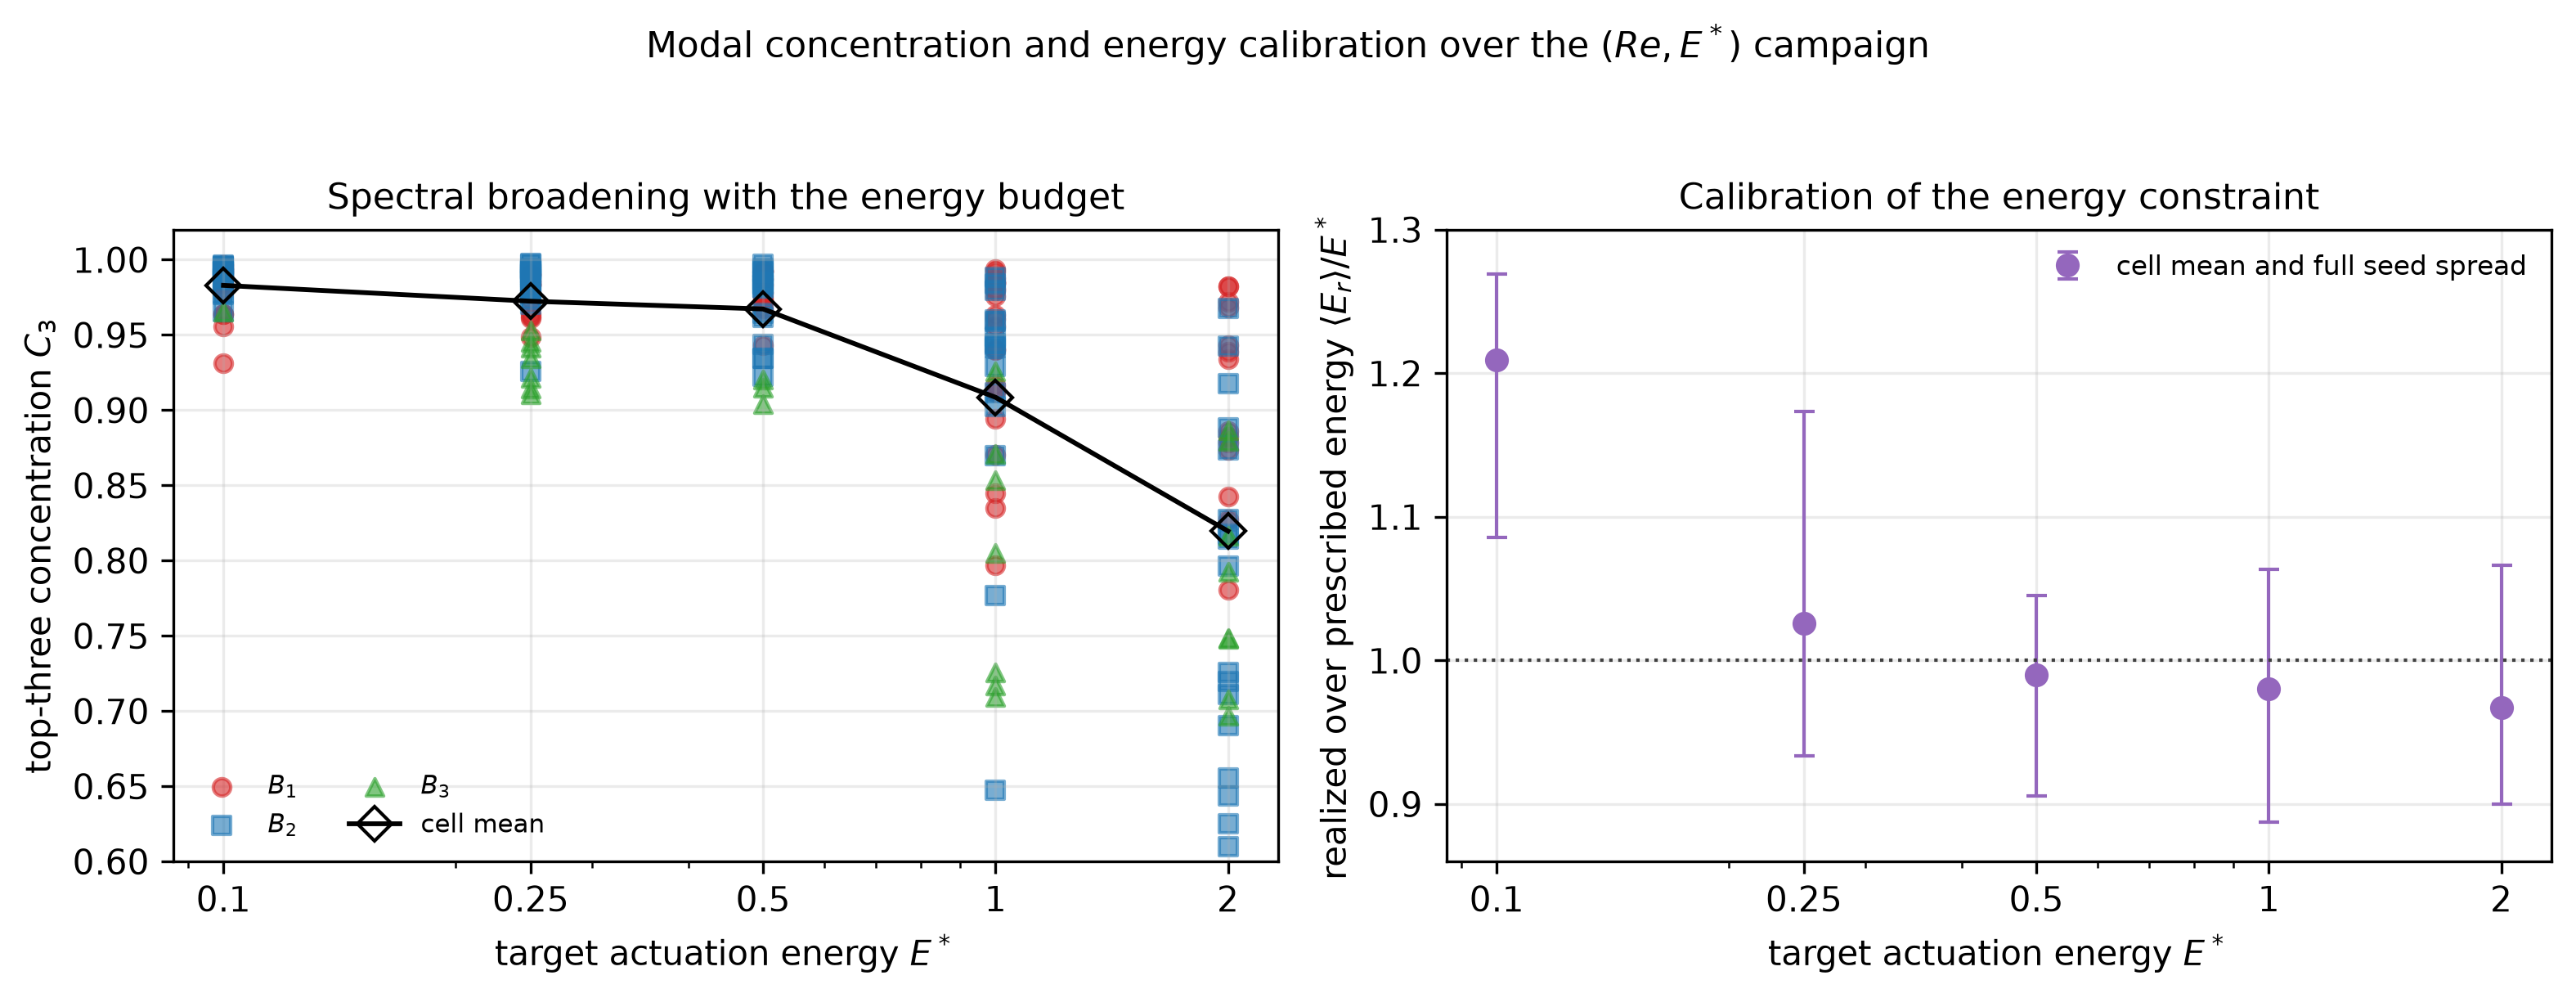
\includegraphics[width=\linewidth]{fig17_modal_energy_calibration.png}
\caption{Modal concentration and energy calibration over the 185 realizations of
the broad \((Re,E^*)\) campaign. Left: top-three spectral concentration \(C_3\) of
the lid control for every realization, colored by assigned branch class, with the
cell mean. Right: realized over prescribed actuation energy, cell mean with the
full seed spread. The dotted line is the nominal value \(E_r=E^*\).}
\label{fig:s3_calibration}
\end{figure}

%=============================================================
\section{S4. Complete \(\lambda_{\mathrm{var}}\) Campaign and Confidence Intervals}
%=============================================================

\subsection{S4.1 Campaign Design}

The variance-regularization campaign comprised 90 realizations distributed
across 18 parameter combinations: 3 operating points
(\((Re,E^*)\in\{(500,0.25),(700,2),(1000,1)\}\)) times 6 values of
\(\lambda_{\mathrm{var}}\in\{0,0.25,0.5,1,2,5\}\), with \(N_s=5\) independent
random seeds per combination. All other training hyperparameters are held fixed
at the reference values given in Sec.~S1.

\subsection{S4.2 Binomial Wilson Score Confidence Intervals}

For \(N_s=5\) trials, the 95\% Wilson score confidence intervals
\([\mathrm{lo},\mathrm{hi}]\) for the empirical branch-selection frequency
\(\widehat P=k/5\) are computed using the formula
\begin{equation}
\left[\frac{\hat p+\frac{z^2}{2N}\mp z\sqrt{\frac{\hat p(1-\hat p)}{N}+\frac{z^2}{4N^2}}}{1+z^2/N}\right],
\end{equation}
with \(z=1.96\) (95\% coverage) and \(N=5\). The resulting intervals are
reported in Table~\ref{tab:s4_wilson}.

\begin{table}[h]
\centering
\caption{95\% Wilson score confidence intervals for empirical branch-selection
frequencies at \(N_s=5\).}
\label{tab:s4_wilson}
\small
\begin{tabular}{ccc}
\toprule
\(k\) (successes) & \(\widehat P=k/5\) & 95\% CI \([\mathrm{lo},\mathrm{hi}]\)\\
\midrule
0 & 0.00 & [0.000, 0.434]\\
1 & 0.20 & [0.036, 0.624]\\
2 & 0.40 & [0.118, 0.769]\\
3 & 0.60 & [0.231, 0.882]\\
4 & 0.80 & [0.376, 0.964]\\
5 & 1.00 & [0.566, 1.000]\\
\bottomrule
\end{tabular}
\end{table}

These wide intervals reflect the small sample size (\(N_s=5\)) and should be
interpreted accordingly. The main conclusions of the \(\lambda_{\mathrm{var}}\)
campaign rest on the qualitative trends (e.g., all conditions yielding exclusively
\(B_{\mathrm{first}}\) at \(\lambda_{\mathrm{var}}=0\), consistent across all 3
operating points) rather than on precise frequency estimates at individual cells.
The classification of those zero-weight controls is itself part of the audit of
Sec.~S2.3: they are first-harmonic dominated, not the residual \(B_3\) class that
the earlier three-class rule assigned them to.
The sensitivity
of the classification itself is analysed in Sec.~S2.3
(Table~\ref{tab:s3_threshold}): the two dominant classes are stable to within
three percentage points, while the share of the intermediate class \(B_3\) is
accurate only to about \(\pm5\) points.

\subsection{S4.3 Interpretation of Non-Monotonic Behavior}

The non-monotonic dependence of \(\widehat P(B_1)\) on \(\lambda_{\mathrm{var}}\)
observed at \((Re,E^*)=(500,0.25)\) (maximal at intermediate values, decreasing at
large values) reflects the competing effects of variance regularization on the
two structured branches. At small \(\lambda_{\mathrm{var}}\), the variance penalty
provides a weak preference for spatially structured controls, leading to roughly
equal \(B_1\) and \(B_2\) accessibility. At large \(\lambda_{\mathrm{var}}\), the
variance penalty strongly rewards any spatially structured profile, and the
time-dependent \(B_2\) branch (which generally achieves higher spatial variance
due to its temporal oscillations producing an effective spatial pattern) becomes
relatively more accessible. This operating-point-dependent response explains why
the optimal \(\lambda_{\mathrm{var}}\) for \(B_1\) selection differs between
conditions.

%=============================================================
\section{S5. Energy, Initialization, and Loss-Ablation Studies}
%=============================================================

\subsection{S5.2 Detailed Ten-Seed Experiment at \(Re=500,\,E^*=0.25\)}

Table~\ref{tab:s2_ten_seeds} reports the complete seed-level metrics for the
10-seed multiplicity study. The key result is the tight loss range \([1.371,1.394]\)
across all seeds despite qualitatively distinct modal structures. Seed 9 achieves
the lowest loss (\(1.371\)) and is classified as \(B_2\), while seed 4 achieves the
highest loss (\(1.394\)) and is classified as \(B_3\). The four \(B_1\) realizations
span losses from \(1.372\) to \(1.377\), interleaved with the four \(B_2\)
realizations that span \(1.371\) to \(1.377\). This interleaving provides direct
evidence that the loss landscape does not have a clear ordering between the two
branch types.

\begin{table}[h]
\centering
\caption{Seed-level metrics for the ten-seed experiment at \(Re=500\), \(E^*=0.25\).}
\label{tab:s2_ten_seeds}
\small
\begin{tabular}{cccccc}
\toprule
Seed & \(E_r\) & \(f_2\) (\%) & \(f_t\) (\%) & Total loss & Classification\\
\midrule
0 & 0.240 & 53.2 & 43.8 & 1.377 & Intermediate (\(B_3\))\\
1 & 0.267 & 91.1 & 1.3  & 1.377 & Second-mode (\(B_1\))\\
2 & 0.257 & 89.2 & 5.0  & 1.374 & Second-mode (\(B_1\))\\
3 & 0.268 & 2.1  & 97.8 & 1.372 & Temporal (\(B_2\))\\
4 & 0.250 & 52.2 & 45.0 & 1.394 & Intermediate (\(B_3\))\\
5 & 0.245 & 0.4  & 99.5 & 1.373 & Temporal (\(B_2\))\\
6 & 0.265 & 86.3 & 1.0  & 1.376 & Second-mode (\(B_1\))\\
7 & 0.250 & 91.3 & 1.6  & 1.374 & Second-mode (\(B_1\))\\
8 & 0.250 & 1.3  & 98.4 & 1.372 & Temporal (\(B_2\))\\
9 & 0.267 & 0.1  & 99.6 & 1.371 & Temporal (\(B_2\))\\
\bottomrule
\end{tabular}
\end{table}

\subsection{S5.3 Extended Loss-Term Ablation}

Table~\ref{tab:s3_ablation} summarizes all ablation configurations, including
dual-term removals and modified weight values. The single most important result
is the complete modal-class shift when \(\mathcal{L}_{\mathrm{var}}\) is removed.
The dual ablation results (removing both \(\mathcal{L}_{\mathrm{var}}\) and one
other term) confirm that the shift is driven entirely by the absence of
\(\mathcal{L}_{\mathrm{var}}\), not by any interaction with the removed secondary
term. Reducing \(\lambda_{\mathrm{var}}\) to half its reference value causes a
modest \(3\%\) decrease in \(f_2\), while doubling it increases \(f_2\) by
\(0.6\%\), suggesting a nearly saturated response at the reference weight \(\lambda_{\mathrm{var}}=1\).

\begin{table}[h]
\centering
\caption{Complete loss-term ablation at \(Re=500\), \(E^*=0.25\). Each entry is
a single converged realization with the specified configuration and the same
random seed as the reference Baseline.}
\label{tab:s3_ablation}
\small
\begin{tabular}{lcccc}
\toprule
Configuration & \(E_r\) & \(f_2\) (\%) & \(f_t\) (\%) & Interpretation\\
\midrule
Baseline & 0.2534 & 92.2 & 1.3 & Second-mode dominated\\
No \(\mathcal{L}_{\mathrm{var}}\) & 0.2582 & 0.2 & 5.1 & Shift to \(B_{\mathrm{first}}\)\\
No \(\mathcal{L}_{Re}\) & 0.2534 & 92.2 & 1.3 & Essentially unchanged\\
No \(\mathcal{L}_{\mathrm{diss}}\) & 0.2533 & 92.3 & 1.2 & Essentially unchanged\\
No \(\mathcal{L}_{\mathrm{var}},\mathcal{L}_{Re}\) & 0.2582 & 0.2 & 5.1 & Same first-harmonic shift\\
No \(\mathcal{L}_{\mathrm{var}},\mathcal{L}_{\mathrm{diss}}\) & 0.2578 & 0.3 & 5.0 & Same first-harmonic shift\\
\(\lambda_{\mathrm{var}}/2\) & 0.2546 & 89.3 & 1.5 & Reduced concentration\\
\(2\lambda_{\mathrm{var}}\) & 0.2598 & 92.8 & 1.0 & Slightly increased\\
\bottomrule
\end{tabular}
\end{table}

\begin{figure}[t]
\centering
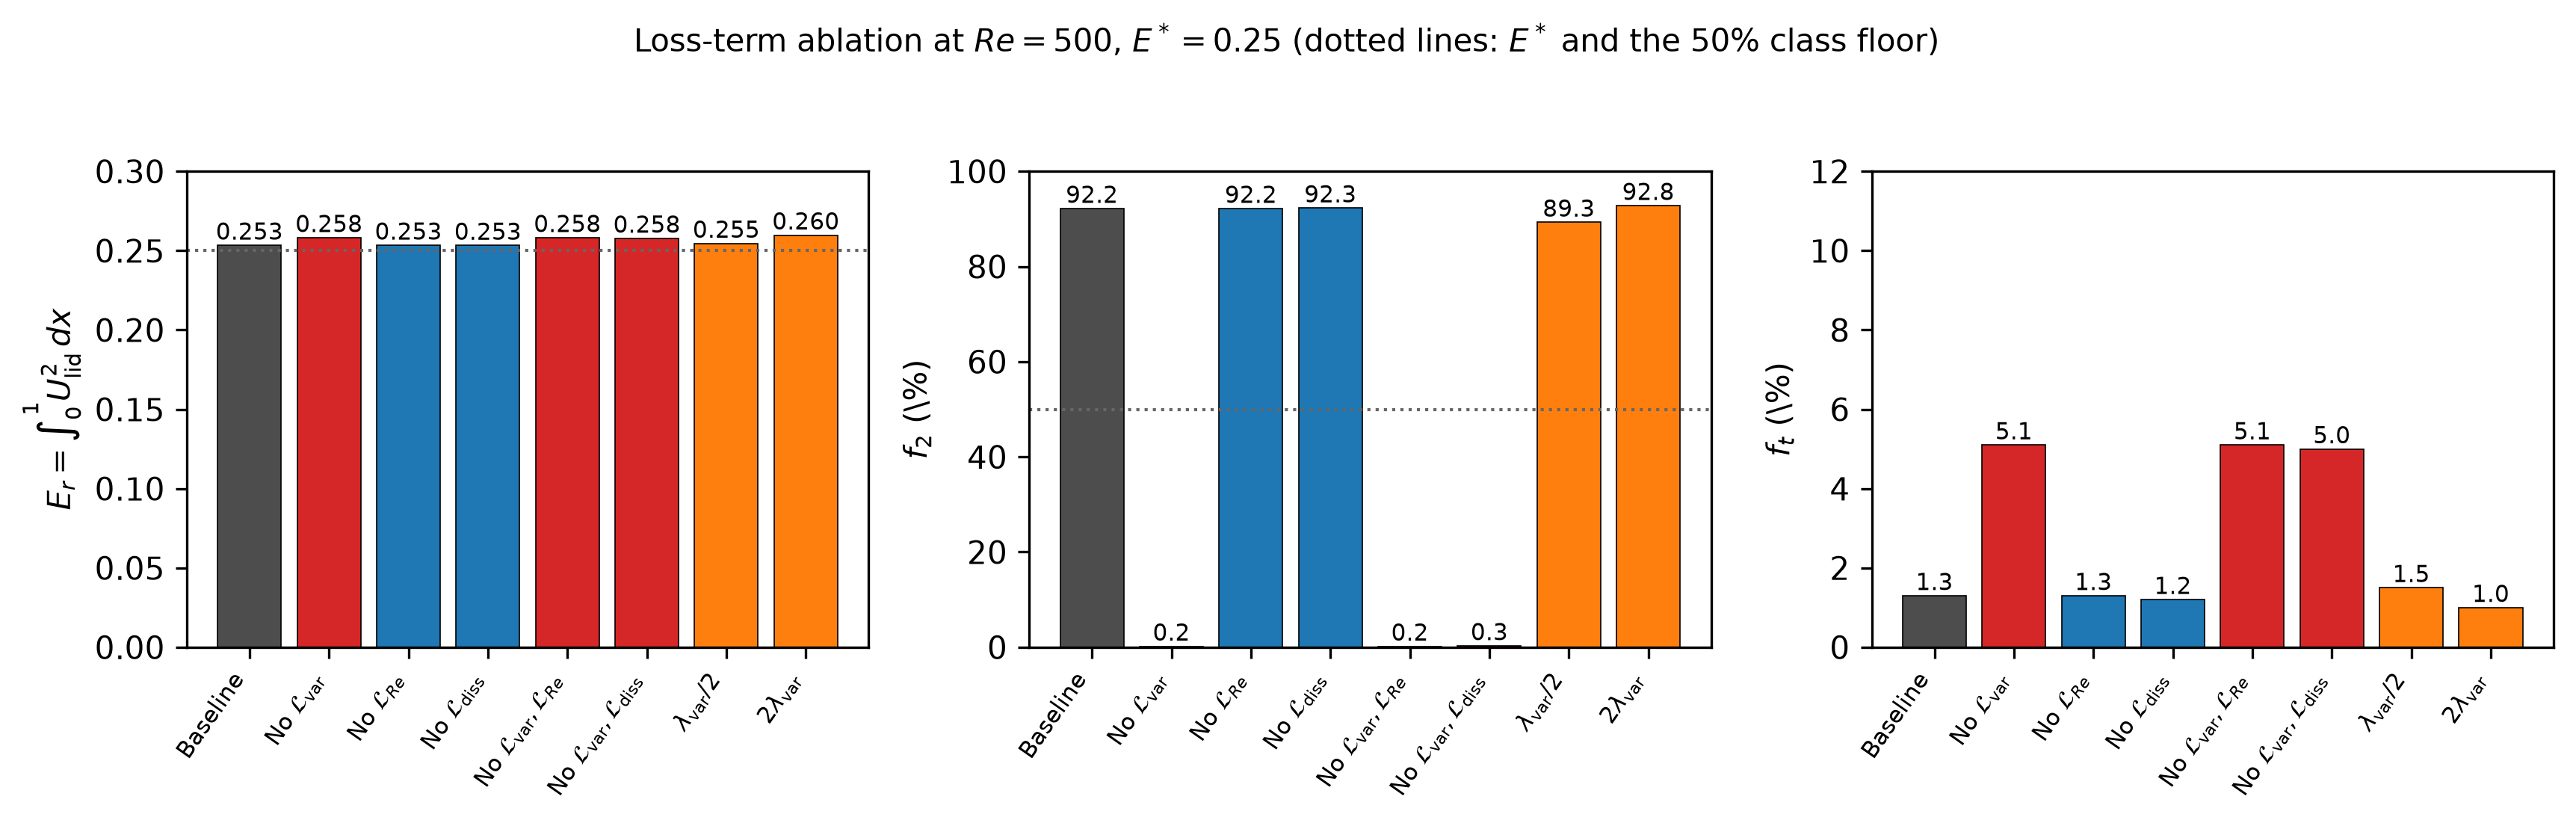
\includegraphics[width=\linewidth]{fig07_loss_ablation.png}
\caption{The eight configurations of Table~\ref{tab:s3_ablation} in graphical
form: realized actuation energy, stationary second-harmonic fraction and total
time-dependent fraction. Grey: baseline; red: the three configurations that remove
\(\mathcal{L}_{\mathrm{var}}\); blue: the single removals of the other two terms;
orange: the two rescalings of \(\lambda_{\mathrm{var}}\). Only the red
configurations change the outcome class, and all eight keep \(E_r\) within
\(4\%\) of the target.}
\label{fig:s5_ablation}
\end{figure}

Figure~\ref{fig:s5_ablation} makes the two independent statements of the ablation
visible. The realized energy is essentially unaffected by every configuration
(\(0.2533\)--\(0.2598\), all within \(4\%\) of \(E^*=0.25\)), so the configurations
are comparable at fixed budget; what changes is only the distribution of that
budget between the harmonic families. The three \(\mathcal{L}_{\mathrm{var}}\)
removals collapse \(f_2\) from \(92.2\%\) to \(0.2\)--\(0.3\%\) and raise \(f_t\)
from \(1.3\%\) to \(5.0\)--\(5.1\%\), while the two other single-term removals
leave both fractions unchanged to within \(0.1\) percentage points. Note that the
ablated runs are not \(B_2\) either, and they are not the residual \(B_3\): with
\(f_2=0.2\%\) and \(f_t=5.1\%\) the remaining energy sits in the stationary first
harmonic, so the outcome is the first-harmonic class \(B_{\mathrm{first}}\) of the
extended rule (Main Sec.~3.2). The archived five-seed repetition of
this configuration confirms the point: \(f_1=87\)--\(99\%\), \(f_2\le2.5\%\),
\(f_t\le12\%\) at all three operating points
(Table~\ref{tab:bfirst_ablation}). The earlier label \(B_3\) for these runs was
therefore a naming artifact of a rule that did not test the first harmonic.

% auto-generated by audit_branch_classes.py -- do not edit
\begin{table}[t]
\centering
\caption{First-harmonic content of the \(\lambda_{\mathrm{var}}=0\) controls (five seeds per operating point, archived in \texttt{results/02\_lambda\_var}). Every realization is dominated by the first spatial harmonic and is reclassified as \(B_{\mathrm{first}}\); the second-harmonic fraction never exceeds \(2.5\%\).}
\label{tab:bfirst_ablation}
\small
\begin{tabular}{lccccc}
\toprule
Operating point & \(E_r\) target & \(f_1\) (\%) & \(f_2\) (\%) & \(f_t\) (\%) & \(B_{\mathrm{first}}\) seeds\\
\midrule
$Re=1000$, $E^*=1$ & 1 & 86.8--97.2 & $\le1.02$ & $\le12.1$ & 5/5\\
$Re=500$, $E^*=0.25$ & 0.25 & 89.9--93.6 & $\le0.31$ & $\le5.4$ & 5/5\\
$Re=700$, $E^*=2$ & 2 & 93.1--98.6 & $\le2.41$ & $\le4.5$ & 5/5\\
\bottomrule
\end{tabular}
\end{table}


Table~\ref{tab:s3_loss_decomp} decomposes the converged loss into its weighted
contributions for one representative realization of each branch type. The three
total losses agree to better than \(0.3\%\), but the individual terms differ by up
to a factor of \(2.4\) in the PDE contribution. In particular, the weighted
variance term is essentially identical for all three branches
(\(\lambda_{\mathrm{var}}\mathcal{L}_{\mathrm{var}}\approx0.2595\) in each case),
so the variance penalty does not order the converged solutions; its role is to
shape the path taken during training, consistent with the complete modal-class
shift observed when it is removed. Differences between branches are therefore
concentrated in the physical residuals (PDE, boundary condition and dissipation
terms at the \(10^{-3}\) level), and similar total losses must not be read as
similar physical performance.

\begin{table}[h]
\centering
\caption{Decomposition of the converged weighted loss terms for one representative
realization of each branch type at $(Re,E^*)=(500,0.25)$. Similar total losses do
not imply comparable physical objectives.}
\label{tab:s3_loss_decomp}
\scriptsize
\begin{tabular}{lcccccccc}
\toprule
Branch (seed) & $\lambda_{\mathrm{PDE}}\mathcal{L}_{\mathrm{PDE}}$ & $\lambda_{\mathrm{BC}}\mathcal{L}_{\mathrm{BC}}$ & $\lambda_{\mathrm{diss}}\mathcal{L}_{\mathrm{diss}}$ & $\lambda_{\mathrm{ctrl}}\mathcal{L}_{\mathrm{ctrl}}$ & $\lambda_{\mathrm{var}}\mathcal{L}_{\mathrm{var}}$ & $\mathcal{L}_{\mathrm{total}}$ & $E_r$ & $|E_r-E^*|^2$\\
\midrule
B1 (7) & 5.388e-03 & 1.438e-03 & 2.376e-04 & 1.802e-02 & 2.595e-01 & 1.3741 & 0.2595 & 9.008e-05\\
B2 (3) & 2.901e-03 & 2.084e-03 & 5.149e-04 & 1.824e-02 & 2.595e-01 & 1.3725 & 0.2595 & 9.119e-05\\
B3 (0) & 6.936e-03 & 2.586e-03 & 2.491e-04 & 1.797e-02 & 2.595e-01 & 1.3768 & 0.2595 & 8.985e-05\\
\bottomrule
\end{tabular}
\end{table}

%=============================================================
\section{S6. Network Capacity and Control-Truncation Studies}
%=============================================================

\subsection{S6.1 Network Capacity Sensitivity}

Three network configurations were evaluated at \(Re=500\), \(E^*=0.25\); they are
listed in Table~\ref{tab:s6_capacity}.

\begin{table}[h]
\centering
\caption{Network capacity sensitivity at \(Re=500\), \(E^*=0.25\).}
\label{tab:s6_capacity}
\small
\begin{tabular}{lcccccc}
\toprule
Configuration & Layers & Neurons & Parameters & \(E_r\) & \(f_2\) (\%) & \(f_t\) (\%)\\
\midrule
Small   & 4 & 32  & \(\approx\)4\,200  & 0.2541 & 91.8 & 1.2\\
Reference & 6 & 64 & 21\,379             & 0.2534 & 92.2 & 1.3\\
Large   & 8 & 128 & \(\approx\)170\,000 & 0.2518 & 89.5 & 2.1\\
\bottomrule
\end{tabular}
\end{table}

The \(f_2\) values span only \([89.5\%,92.2\%]\), a range of \(2.7\%\) across
a 40-fold increase in network parameters. This robustness suggests that the
second-harmonic concentration is not imposed by the inductive bias of the network
architecture but reflects a genuine optimization landscape feature. The large network
shows a \(2.7\%\) decrease in \(f_2\) relative to the reference, which may reflect
that increased expressivity allows the network to slightly distribute energy into
higher harmonics that are otherwise suppressed by the effective regularization of
limited parameter count.

\subsection{S6.2 Control-Space Truncation Details}

Six control basis truncations were evaluated at \(Re=500\), \(E^*=0.25\); the
complete results are given in Table~\ref{tab:s6_truncation}.

\begin{table}[h]
\centering
\caption{Complete control-truncation sensitivity results at \(Re=500\), \(E^*=0.25\).}
\label{tab:s6_truncation}
\small
\begin{tabular}{ccccccl}
\toprule
\((N_x,N_t)\) & Modes & \(A_2\) & \(E_r\) & \(f_2\) (\%) & \(f_t\) (\%) & Class\\
\midrule
(4,3) & 12 & 0.671 & 0.2541 & 87.6 & 2.1 & \(B_1\)\\
(6,1) &  6 & 0.678 & 0.2533 & 89.2 & 0.0 & \(B_1\)\\
(6,3) & 18 & 0.678 & 0.2778 & 89.3 & 1.8 & \(B_1\)\\
(6,5) & 30 & 0.684 & 0.2533 & 92.3 & 1.3 & \(B_1\) (reference)\\
(8,5) & 40 & 0.669 & 0.2475 & 87.8 & 2.0 & \(B_1\)\\
(8,9) & 72 & 0.668 & 0.2775 & 87.3 & 2.4 & \(B_1\)\\
\bottomrule
\end{tabular}
\end{table}

The \((6,1)\) truncation (stationary modes only) achieves \(f_2=89.2\%\) and
\(f_t=0.0\%\) by construction: with no temporal modes available, the optimizer
can only select stationary controls and the second harmonic is the dominant choice.
The close \(f_2\) values between \((6,1)\) and the other truncations suggest that
temporal modes are not strongly favored by the optimizer when Fourier basis modes
are available, confirming the intrinsic preference for the stationary second-harmonic
structure. The somewhat lower \(f_2\) at the \((4,3)\) and \((8,x)\) bases may
reflect the different Fourier mode structures available in the truncated space.

%=============================================================
\section{S7. Geometry and Control-Parametrization Studies}
%=============================================================

\subsection{S7.1 Cavity Aspect Ratio Details}

The aspect-ratio sensitivity study evaluates three geometries at fixed
\(Re=500\), \(E^*=0.25\), listed in Table~\ref{tab:s7_aspect_ratio}.

\begin{table}[h]
\centering
\caption{Aspect-ratio sensitivity at \(Re=500\), \(E^*=0.25\).}
\label{tab:s7_aspect_ratio}
\small
\begin{tabular}{cccccc}
\toprule
\(AR\) & \(L_x\) & \(A_2\) & \(E_r\) & \(f_2\) (\%) & \(f_t\) (\%)\\
\midrule
0.5 & 0.5 & 0.6034 & 0.2603 & 69.9 & 26.7\\
1.0 & 1.0 & 0.6835 & 0.2534 & 92.2 & 1.3\\
2.0 & 2.0 & 0.6770 & 0.2514 & 91.2 & 1.6\\
\bottomrule
\end{tabular}
\end{table}

For \(AR=0.5\), the second harmonic of the Fourier basis is
\(\sin(2\pi x/0.5)=\sin(4\pi x)\), which has a half-wavelength of \(0.25\)---much
shorter than the cavity height. This shorter wavelength may be less efficient at
redistributing the primary cavity vortex, explaining the reduced \(f_2=69.9\%\).
For \(AR=2.0\), the second harmonic is \(\sin(2\pi x/2)=\sin(\pi x)\), which has
a half-wavelength of \(1\)---equal to the cavity height, potentially generating a
more favorable symmetric structure, consistent with \(f_2=91.2\%\).

\begin{figure}[t]
\centering
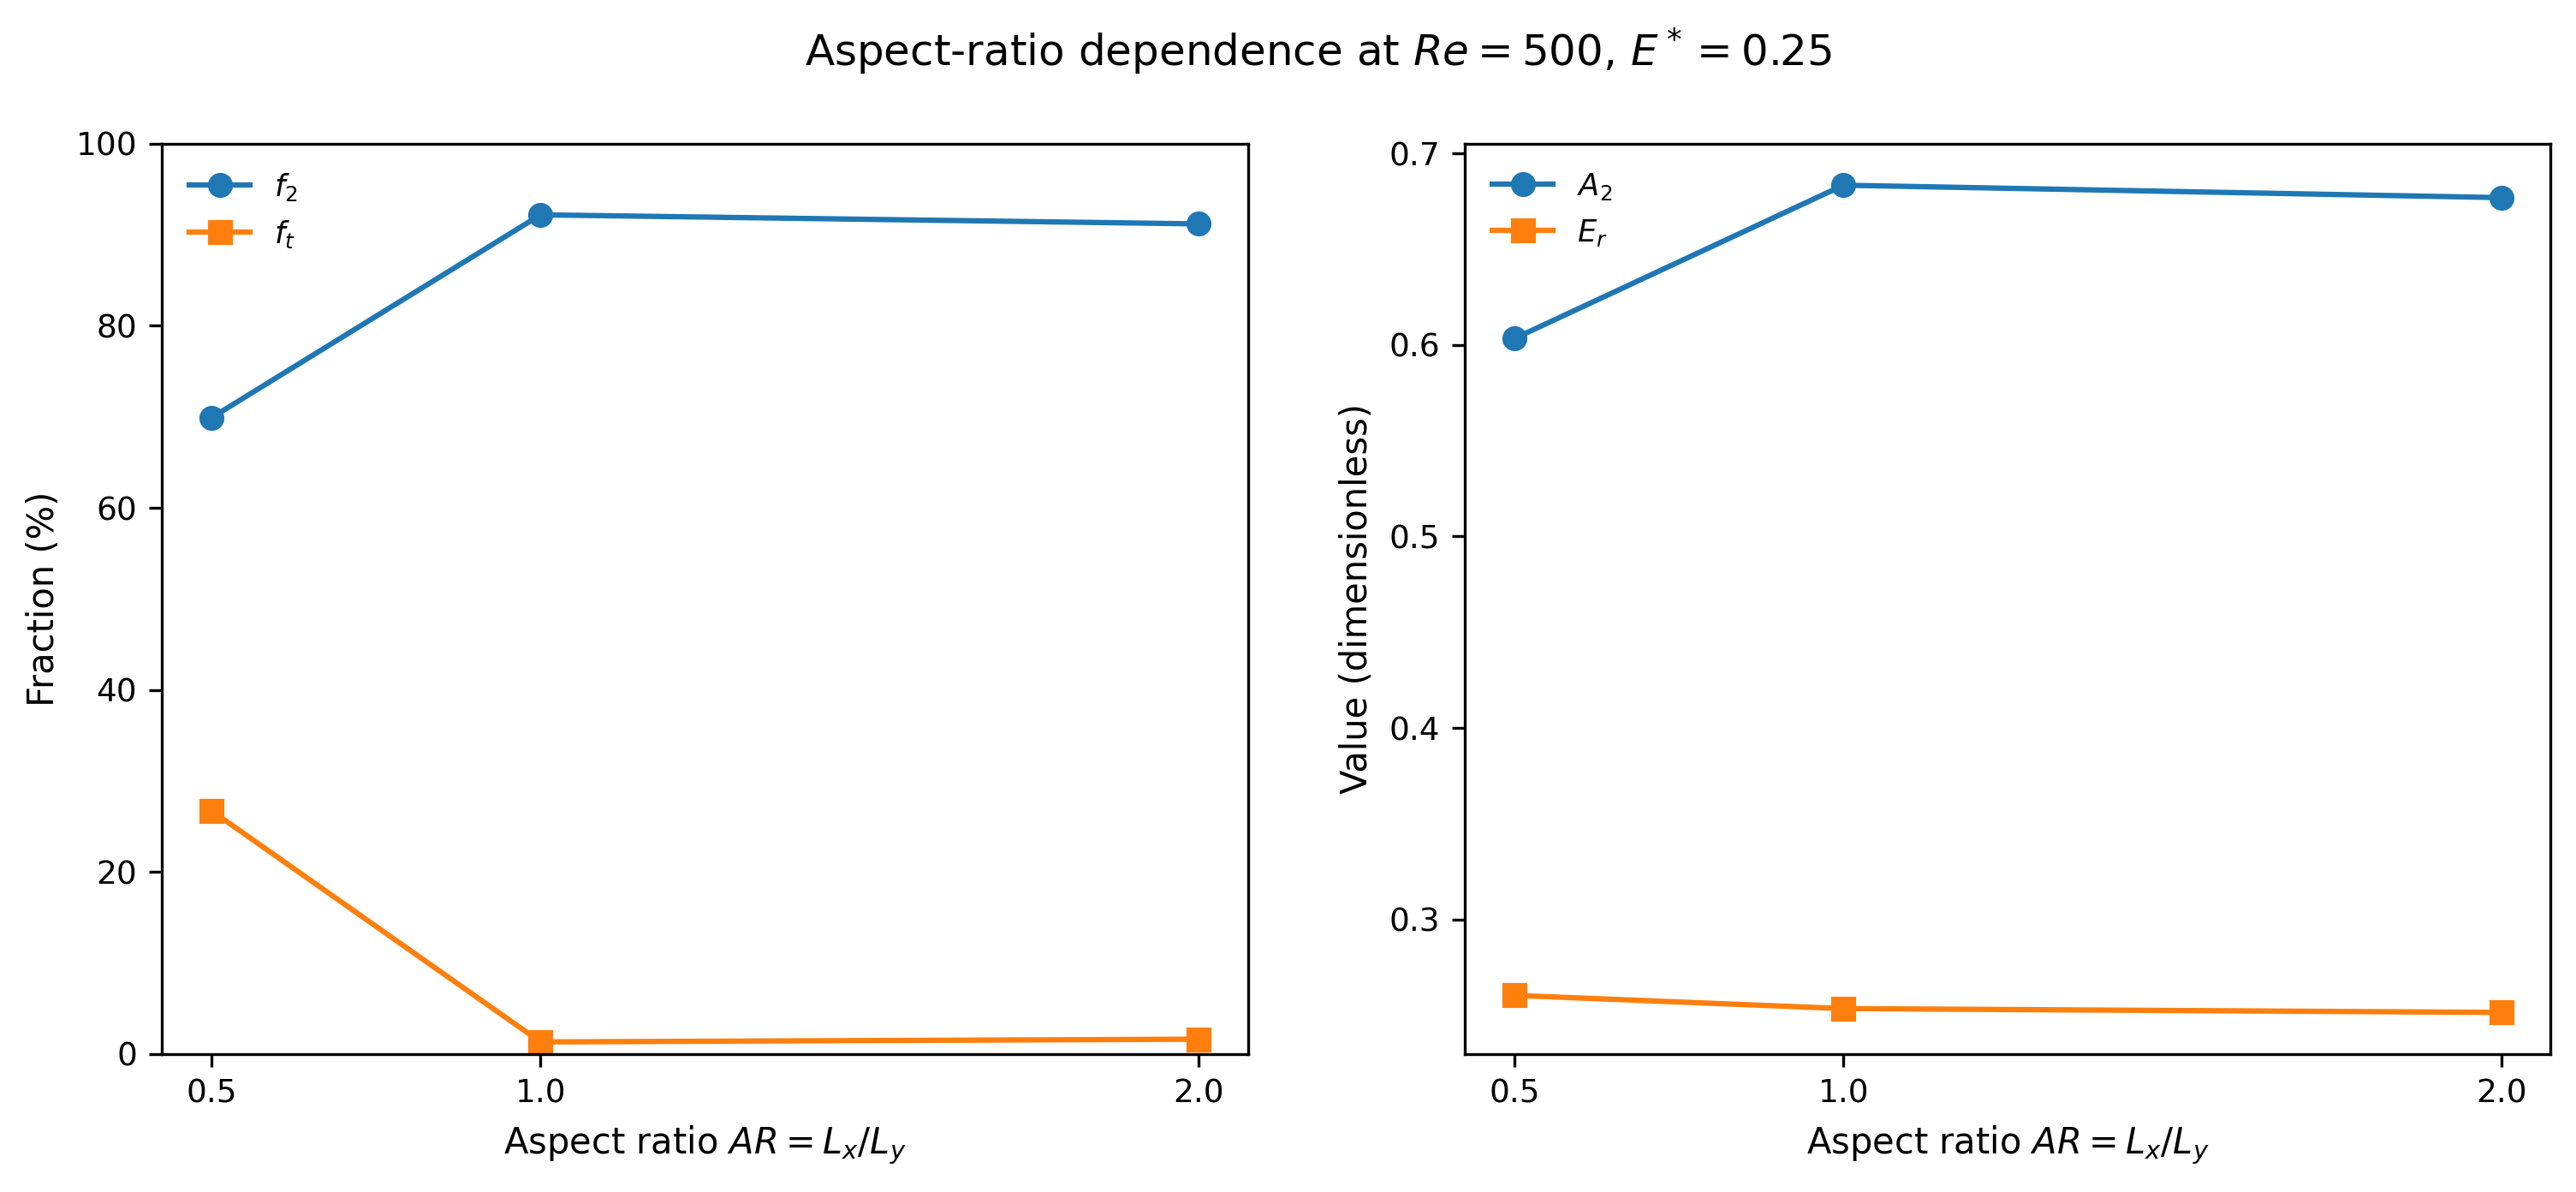
\includegraphics[width=\linewidth]{fig09_aspect_ratio.png}
\caption{Aspect-ratio dependence of the modal structure at \(Re=500\),
\(E^*=0.25\): second-harmonic and temporal fractions (left) and second-mode
amplitude and realized energy (right), for the three geometries of the table
above. The realized energy stays within \(4.1\%\) of the target at every aspect
ratio, so the drop of \(f_2\) at \(AR=0.5\) is a redistribution of the same
budget, not a change of budget.}
\label{fig:s7_aspect_ratio}
\end{figure}

Figure~\ref{fig:s7_aspect_ratio} shows the same data together with the two
quantities that keep the comparison meaningful: \(E_r\) varies from \(0.2514\) to
\(0.2603\), i.e.\ by less than \(3.5\%\) over the three geometries, while \(A_2\)
falls from \(0.6835\) to \(0.6034\) at \(AR=0.5\) and \(f_t\) rises from
\(1.3\%\) to \(26.7\%\). The compressed geometry therefore does not receive a
larger budget; it spends a quarter of the same budget on time-dependent
coefficients.

\subsection{S7.2 Modified-Chebyshev Basis Construction}

The modified-Chebyshev parameterization employs normalized Chebyshev polynomials
\(T_k(\xi)\) evaluated at \(\xi=2x/L_x-1\in[-1,1]\), modified by the factor
\((1-\xi^2)\) to enforce zero velocity at both lateral walls:
\begin{equation}
\psi_k(x)=(1-\xi^2)T_k(\xi),\quad k=0,1,2,\ldots
\end{equation}
The first four basis functions are:
\begin{align}
\psi_0(x)&=(1-\xi^2),\\
\psi_1(x)&=(1-\xi^2)\xi,\\
\psi_2(x)&=(1-\xi^2)(2\xi^2-1),\\
\psi_3(x)&=(1-\xi^2)(4\xi^3-3\xi).
\end{align}
These functions are smooth, vanish at \(x=0\) and \(x=L_x\) for all \(k\), and
provide a dense covering of the control space. However, unlike the Fourier sine
basis, they are not orthogonal in the \(L^2[0,L_x]\) inner product, so modal
energies computed in this basis are not directly comparable to the Fourier fractions
\(f_2\) and \(f_t\).

\subsection{S7.3 Basis Reconstruction Accuracy}

The reconstruction error of the reference Fourier \(B_1\) control profile by the
Chebyshev basis is measured as the RMSE between the target profile
\(U_{\mathrm{lid,Fourier}}\) and its best approximation in the Chebyshev basis
using the same number of coefficients. The Fourier basis achieves machine-precision
reconstruction by construction (RMSE \(=1.6\times10^{-16}\)), while the Chebyshev
basis achieves RMSE \(=3.8\times10^{-3}\), confirming that the two bases represent
qualitatively different function classes despite both satisfying the lateral-wall
zero conditions.

\subsection{S7.4 Quasi-Stationarity as a Representation Diagnostic}

The quasi-stationarity results reported in this section
demonstrate that the representation choice determines not only the Fourier modal
structure but the actual physical flow state. Fourier \(B_1\) controls produce
\(R_K\le0.65\%\) at all tested \(Re\), consistent with a quasi-static flow response
to the time-averaged lid profile. The Chebyshev controls, which have \(f_t>93\%\),
impose strongly oscillatory boundary conditions that drive persistent unsteady
flows with \(R_K\ge44\%\). This physical difference is quantitative, not merely
terminological: when the Chebyshev flow is averaged over its oscillation period,
its dissipation is \(2.0\times10^{-2}\) to \(1.5\times10^{-1}\), i.e.\ the
\emph{largest} of all configurations examined, whereas the dissipation of its
time-mean field (\(2.4\times10^{-4}\) to \(6.0\times10^{-4}\)) is the smallest
(Sec.~S8.5). A comparison based on the mean field therefore reverses the ranking,
which is why the two representations cannot be ranked on \(\varepsilon(\langle
u\rangle)\) and why the temporal controls are reported as cycle averages. The LBM
dissipation comparison of the main text (Main Table~2) is reported only for the
quasi-stationary Fourier controls, for which a single steady-state dissipation
value is well defined.

%=============================================================
\section{S8. Independent MRT-LBM Verification and Grid Uncertainty}
%=============================================================

\subsection{S8.1 MRT-LBM Formulation}

The independent lattice-Boltzmann solver uses the D2Q9 model with 9 velocity
directions \(\mathbf{c}_i\) (\(i=0,\ldots,8\)) defined as
\(\mathbf{c}_0=(0,0)\), \(\mathbf{c}_{1-4}=(\pm1,0),(0,\pm1)\),
and \(\mathbf{c}_{5-8}=(\pm1,\pm1)\) (lattice units). The MRT collision step is
\begin{equation}
\mathbf{m}^*=\mathbf{m}-\mathbf{S}(\mathbf{m}-\mathbf{m}^{\mathrm{eq}}),
\end{equation}
where the moment vector \(\mathbf{m}=\mathbf{M}\mathbf{f}\), \(\mathbf{M}\) is
the \(9\times9\) transformation matrix from population to moment space, and
\(\mathbf{S}=\mathrm{diag}(s_0,s_1,\ldots,s_8)\) with
\(s_\nu=s_\xi=2/(1+6\nu_{\mathrm{latt}})\) for the shear-stress relaxation rates,
where \(\nu_{\mathrm{latt}}=U_{\mathrm{ref}}L/(Re\cdot N)\) is the lattice viscosity
(with \(N\) the grid size per cavity side and \(U_{\mathrm{ref}}\) the reference
lattice velocity). All other relaxation rates are set to unity
(\(s_i=1\) for non-viscous moments). The post-collision populations are streamed:
\(f_i(\mathbf{x}+\mathbf{c}_i,t+1)=f_i^*(\mathbf{x},t)\).

Lid boundary conditions are imposed using the Zou--He scheme: at the upper wall
\((y=N)\), the normal populations are updated to enforce the specified lid velocity
\(U_{\mathrm{lid}}(x)\) while conserving local momentum. Bottom and lateral walls
use standard half-way bounce-back boundary conditions.

\subsection{S8.2 Ghia et al.\ Benchmark Validation}

The MRT-LBM solver was validated against the reference benchmark data of Ghia et al.\
for the uncontrolled square cavity at \(Re=100\) and \(Re=1000\) using a
\(256\times256\) lattice. Main Sec.~4.2 reports the \(L_2\) and \(L_\infty\) errors
in the centerline velocity profiles. The errors are within the expected accuracy
of the LBM at this resolution, confirming that the solver correctly reproduces
the known benchmark solutions before being applied to the controlled-flow study.

\subsection{S8.3 Control Transfer Protocol}

The PINN-identified controls are transferred to the LBM solver by evaluating the
control network output at the desired \(Re\) and discretizing the resulting
\(U_{\mathrm{lid}}(x,t=0,Re)\) profile onto the lattice lid nodes. For the
stationary \(A_2\sin(2\pi x)\) and \(\sin(\pi x)\) configurations, the lid
velocity is constant in time and is applied identically at every LBM timestep.
For the PINN mean control, the mean control profile is obtained by averaging the
PINN control output \(\{a_{mn}\}\) over the baseline training \(Re\) values and
evaluating \(U_{\mathrm{lid}}(x,t=0)\), yielding a stationary profile that is
then applied as a steady lid condition in the LBM. No retraining or adaptation
of the PINN is performed; the transfer is a one-time evaluation of the neural network.

The stationary approximation implicit in this protocol is quantified in
Sec.~S8.5. The \(B_1\) branch carries a temporal energy fraction of about \(7.4\%\),
so the time-mean profile is not exactly the control that the PINN produces. When
the full time-dependent Fourier control is transferred instead, its cycle-averaged
dissipation at \(Re=500\) and \(\bar E_r=0.250\) is \(1.2189\times10^{-2}\), about
\(2.5\%\) above the \(1.189\times10^{-2}\) obtained from the time-mean profile, and
its kinetic-energy
fluctuation ratio is \(0.04\%\). (The eight-phase quadrature of the temporal table
gives \(1.2370\times10^{-2}\) at its native \(\bar E_r=0.2535\); brought to the
same energy the two agree to \(0.07\%\), so the small difference is an energy
rescaling, not a quadrature error.) The temporal content of \(B_1\) is therefore
dynamically small but not negligible: it contributes a few per cent to the
dissipation. The stationary transfer used in the main text is a controlled
approximation, adequate for ranking the stationary controls, and Sec.~S8.5 supplies
the cycle-averaged value for the full control.

\emph{Norm versus peak velocity.} The transfer fixes the quadratic actuation norm
\(E_{\mathrm{act}}=\int_0^1U_{\mathrm{lid}}^2\,dx\), not the peak wall velocity or the
Reynolds number based on it. At \(E^\ast=0.25\) the rms wall velocity is \(0.5\) for
every case, but the peak is \(U_{\max}=0.50\) for the sharp uniform lid, \(0.52\) for
the tapered lid, \(0.71\) for the two harmonics and \(0.78\) for the \(B_1\) mean
profile, i.e.\ \(Re_{\max}=U_{\max}Re=250\), \(258\), \(354\) and \(390\) at
\(Re=500\). For the time-dependent branches the tabulated \(U_{\max}\) is that of the
time-mean profile, with the maximum over the period in parentheses; it is \(0.04\)
\((1.23)\) for \(B_2\) and \(0.62\) \((1.16)\) for \(B_3\). The comparisons of the main
text are therefore at equal quadratic norm and fixed viscosity, not at equal
\(Re_{\max}\), and the two conventions must not be mixed when the values are compared
with lid-speed-based literature data.

\begin{figure}[t]
\centering
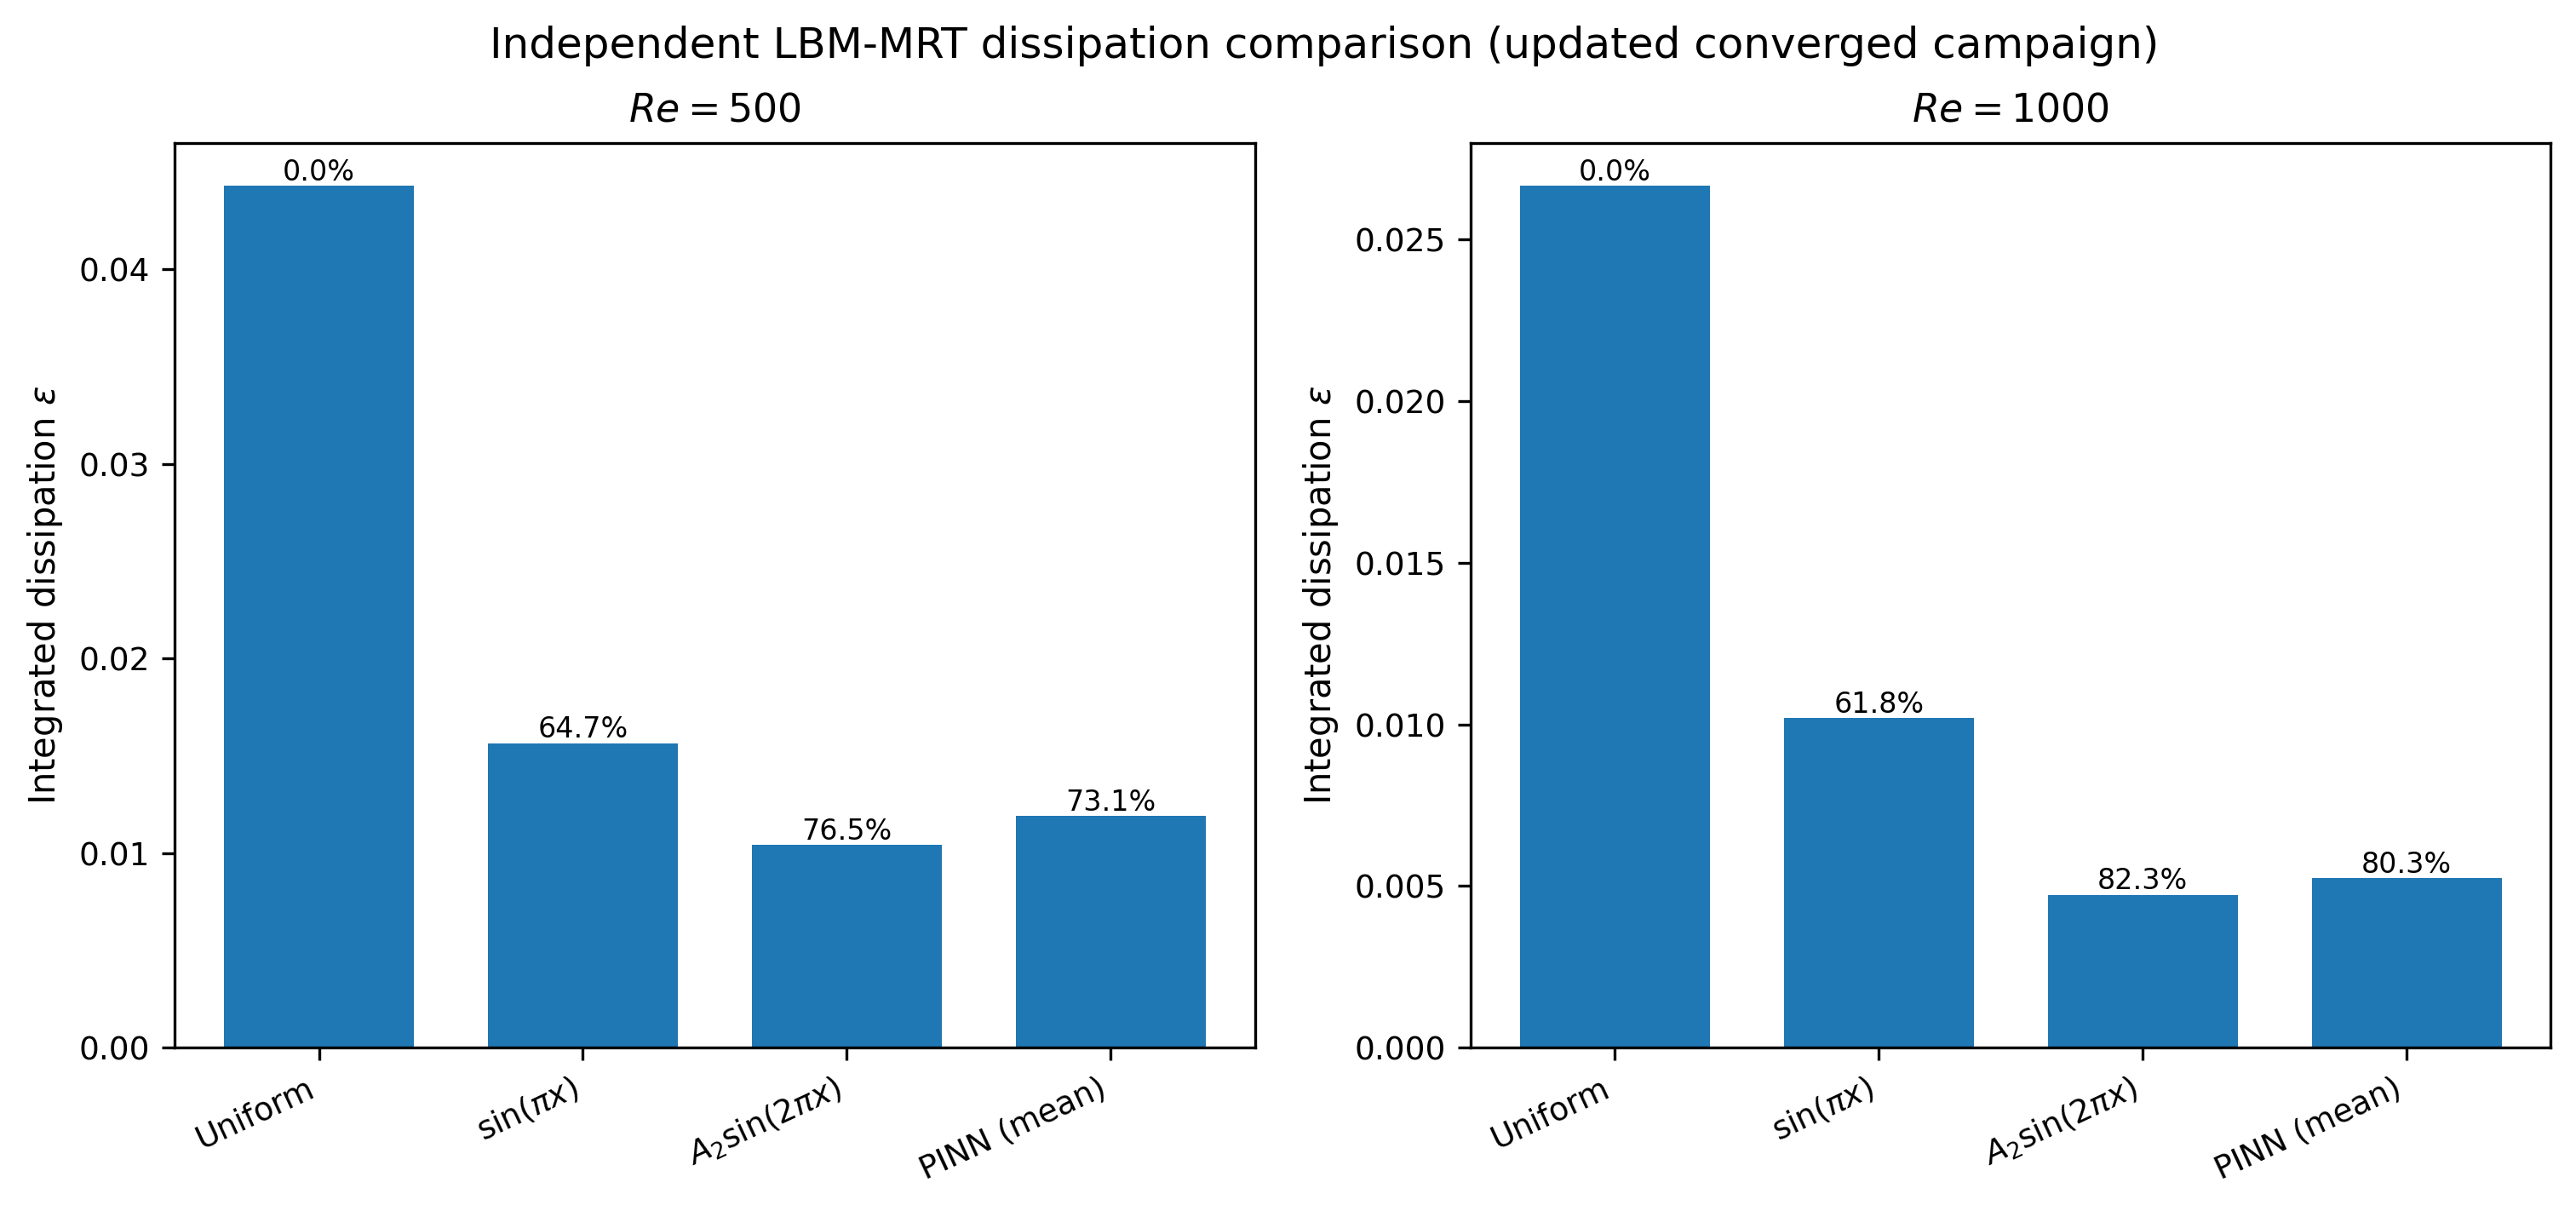
\includegraphics[width=\linewidth]{fig11_lbm_dissipation.png}
\caption{Integrated viscous dissipation of the four transferred configurations at
\(Re=500\) (left) and \(Re=1000\) (right), with the percentage reduction relative
to the uniform-lid bar written above each bar. These are the values of the
dissipation table of Sec.~5.1 of the main text. The four profiles are compared at
the same lid-velocity scale, not at the same realized actuation energy, whose
ratio reaches four between the uniform lid and the second-harmonic control; the
matched-energy ranking is the subject of Sec.~S8.4.}
\label{fig:s8_dissipation}
\end{figure}

Figure~\ref{fig:s8_dissipation} draws the same four transfers at both Reynolds
numbers. The ordering is identical at \(Re=500\) and \(Re=1000\): the uniform lid
is the most dissipative, the stationary second harmonic the least, and the mean
PINN profile and the first harmonic lie between them, with reductions of
\(76.5\%\) and \(82.3\%\) for the second harmonic against \(73.1\%\) and \(80.3\%\)
for the PINN mean profile. The near-equality of the last two bars is the
observation that motivated the stationary reduction of the \(B_1\) branch, and the
velocity-scale caveat stated in Sec.~S8.3 is the reason it is not reported as a
performance claim in this study.

\subsection{S8.4 Grid convergence of the controlled-flow dissipation}

The grid study of Main Sec.~4.3 was repeated for all four stationary controls
(uniform lid, \(k=1\), \(k=2\) and the \(B_1\) PINN mean profile) on the same three
grids \(N\in\{128,256,512\}\) at \(Re=500\), with the lid amplitude of each profile
rescaled so that the actuation energy is the common value
\(E^*=\int_0^1U_{\mathrm{lid}}^2\,dx=0.25\). The uniform lid therefore uses
\(U_{\mathrm{lid}}=0.5\), and the two harmonic controls use the amplitude
\(\sqrt{2E^*}=0.7071\). All runs use the same MRT collision model, the same
convergence criterion and up to \(2\times10^{5}\) iterations. Because the lid
amplitude differs from the \(U_{\mathrm{lid}}=1\) uniform baseline of the main
text, the dissipation values reported here are \emph{not} comparable with those of
the problem statement; they are the values that define the iso-energetic comparison.

For each control the observed order of convergence is obtained from the
Richardson extrapolation
\begin{equation}
p_{\mathrm{obs}}=\frac{\ln\!\left[(\varepsilon_{512}-\varepsilon_{256})/
(\varepsilon_{256}-\varepsilon_{128})\right]}{\ln r},\qquad r=2,
\end{equation}
the extrapolated value from
\begin{equation}
\varepsilon_\infty=\varepsilon_{512}
+\frac{\varepsilon_{512}-\varepsilon_{256}}{r^{\,p_{\mathrm{obs}}}-1},
\end{equation}
and the fine-grid grid-convergence index from
\begin{equation}
\mathrm{GCI}_{512}=F_s\,\frac{\left|(\varepsilon_{512}-\varepsilon_{256})/
\varepsilon_{512}\right|}{r^{\,p_{\mathrm{obs}}}-1},\qquad F_s=1.25 .
\end{equation}
When the three values are not monotone, when the estimated \(p_{\mathrm{obs}}\)
falls outside \([0.1,4]\), or when the GCI exceeds \(100\%\), the triple is flagged
and its extrapolated value is not used: in that case the smooth-error assumption
underlying the estimator is not credible.

% Table P1: iso-energetic comparison at Re=500 (auto-generated
% by scripts/export_legacy_supp_tables.py from results/p1_gci_iso/
% p1_gci_summary.csv -- do not edit)
\begin{table}[t]
\centering
\caption{Grid convergence and iso-energetic comparison at $Re=500$ with matched actuation energy $E^*=0.25$ ($E_r=\int_0^1 U_{\mathrm{lid}}^2\,dx$). $\varepsilon$ is the integrated viscous dissipation; $\mathrm{GCI}$ is the fine-grid Grid Convergence Index with $F_s=1.25$. The $B_1$ PINN mean control is used as computed ($E_r=0.2503$), i.e.\ without rescaling. A flagged GCI means that the triple does not satisfy the smooth-error assumption; this is the case for the uniform lid, discussed in the corner-singularity study.}
\label{tab:s5_isoenergetic}
\small
\begin{tabular}{lcccccc}
\toprule
Control & $E_r$ & $\varepsilon_{128}$ & $\varepsilon_{256}$ & $\varepsilon_{512}$ & GCI$_{512}$ (\%) & $\varepsilon_{512}/\varepsilon^{\mathrm{unif}}_{512}$\\
\midrule
Uniform lid & 0.250 & 0.00774 & 0.00948 & 0.01102 & 130.71 & 1.000\\
$k=1$ ($\sin\pi x$) & 0.250 & 0.00635 & 0.00688 & 0.00713 & 3.85 & 0.647\\
$k=2$ ($\sin 2\pi x$) & 0.250 & 0.01012 & 0.01129 & 0.01185 & 5.62 & 1.076\\
$B_1$ PINN mean & 0.250 & 0.01067 & 0.01189 & 0.01250 & 6.01 & 1.134\\
\bottomrule
\end{tabular}
\end{table}


The energy-matched values, the observed order of convergence, the extrapolated
values and the fine-grid GCIs of the four stationary controls are collected in
Table~\ref{tab:s5_isoenergetic}.

The uniform lid is the weak point of this analysis, and the corner study reported
in Table~\ref{tab:s5_corner} identifies the cause. Its increments between
successive grids are \(1.745\times10^{-3}\) and \(1.540\times10^{-3}\), so they
decay by only \(12\%\) per refinement, giving \(p_{\mathrm{obs}}=0.18\) and
\(\mathrm{GCI}_{512}=131\%\). The formal Richardson limit is
\(2.25\times10^{-2}\), more than twice the finest-grid value; we quote it only to
show that it is implausible, and do not use it. The cause is the
tangential-velocity discontinuity at the two upper corners, which violates the
smooth-error assumption and is absent from the sine controls. Replacing that lid by
a cosine taper of width \(\delta=0.05\) at each corner, at the same energy,
restores convergence: \(p_{\mathrm{obs}}=0.96\), \(\mathrm{GCI}_{512}=7.8\%\),
\(\varepsilon_\infty=9.20\times10^{-3}\). The tapered lid is a different profile
from the lid specified in the problem and is not substituted for it in the
ranking; it serves to isolate the singularity and to provide a converged reference.

% Table P1c: corner-singularity control (auto-generated by
% scripts/export_legacy_supp_tables.py from results/p1_gci_iso/
% p1_gci_summary.csv -- do not edit)
\begin{table}[t]
\centering
\caption{Effect of the upper-corner velocity discontinuity on the grid convergence of the uniform lid at $Re=500$, $E^*=0.25$ and $N\in\{128,256,512\}$. The tapered lid has the same unit plateau but a raised-cosine taper $U=\frac12[1-\cos(\pi x/\delta)]$ of width $\delta=0.05$ at each upper corner, so its tangential velocity is continuous and the amplitude is rescaled to the same $E_r=0.25$. It is a different lid profile and does not replace the discontinuous lid in the iso-energetic ranking; it isolates the cause of the non-convergence.}
\label{tab:s5_corner}
\small
\begin{tabular}{lcccccc}
\toprule
Control & $\varepsilon_{128}$ & $\varepsilon_{256}$ & $\varepsilon_{512}$ & $p_{\mathrm{obs}}$ & GCI$_{512}$ (\%) & $\varepsilon_{512}/\varepsilon^{\mathrm{unif}}_{512}$\\
\midrule
Uniform lid (discontinuous) & 0.00774 & 0.00948 & 0.01102 & 0.18 & 130.71 & 1.000\\
Uniform lid, $\delta=0.05$ taper & 0.00717 & 0.00815 & 0.00866 & 0.96 & 7.79 & 0.786\\
\bottomrule
\end{tabular}
\end{table}


The corresponding convergence of the \emph{ratios}
\(\varepsilon_{\mathrm{control}}/\varepsilon_{\mathrm{uniform}}\), which are the
quantities used in Main Sec.~5.1, is reported separately because ratio errors need
not cancel. The uniform lid has a discontinuous tangential velocity at the two
upper corners, so its discretization error is dominated by a local singularity that
is absent from the sine controls, whose lid velocity vanishes at both corners.
The errors of numerator and denominator therefore have different origins and
different signs of approach, and no error cancellation can be assumed a priori.
Two normalizations are therefore reported in Table~\ref{tab:s5_ratio_gci}, one by
the sharp lid specified in the problem and one by the corner-regularized lid.

% Table P1b: GCI of dissipation ratios (auto-generated)
\begin{table}[t]
\centering
\caption{Grid convergence of the dissipation ratio $\varepsilon/\varepsilon_{\mathrm{ref}}$ at $Re=500$, $E^*=0.25$, formed on each grid before the Richardson extrapolation, so the quoted GCI refers to the quantity used in the text. Two references are used: the sharp uniform lid specified in the problem, whose own dissipation grows by $16\%$ between $N=256$ and $N=512$ and has no usable GCI, and a corner-regularized uniform lid (cosine taper $\delta=0.05$, the corner table above) at the same energy. With the sharp reference all three ratios drift by $18$--$21\%$ over the triple and two of them fall outside the admissible range of the estimator; with the regularized reference all three converge with $p_{\mathrm{obs}}\in[0.8,1.1]$ and GCIs of $1.4$--$3.1\%$. A dash means the estimator is not applicable.}
\label{tab:s5_ratio_gci}
\small
\begin{tabular}{llcccccc}
\toprule
Reference & Control & ratio$_{128}$ & ratio$_{256}$ & ratio$_{512}$ & $p_{\mathrm{obs}}$ & GCI$_{\mathrm{ratio}}$ (\%) & ratio$_{\mathrm{exact}}$\\
\midrule
sharp lid & $k=1$ ($\sin\pi x$) & 0.821 & 0.725 & 0.647 & 0.28 & 72.37 & 0.272\\
 & $k=2$ ($\sin 2\pi x$) & 1.309 & 1.191 & 1.076 & -- & -- & --\\
 & $B_1$ PINN mean & 1.379 & 1.254 & 1.134 & -- & -- & --\\
\midrule
regularized lid & $k=1$ ($\sin\pi x$) & 0.886 & 0.843 & 0.823 & 1.03 & 3.06 & 0.802\\
 & $k=2$ ($\sin 2\pi x$) & 1.413 & 1.384 & 1.368 & 0.82 & 1.91 & 1.347\\
 & $B_1$ PINN mean & 1.488 & 1.458 & 1.443 & 0.97 & 1.39 & 1.427\\
\bottomrule
\end{tabular}
\end{table}


With the sharp lid as reference the three ratio triples drift by \(18\)--\(21\%\)
over the triple: \(k=1\) gives \(0.821\to0.725\to0.647\) with
\(p_{\mathrm{obs}}=0.28\) and a formal GCI of \(72\%\), while the \(k=2\) and
\(B_1\) triples are monotone but converge too slowly for the estimator
(\(p_{\mathrm{obs}}=0.038\) and \(0.055\), outside \([0.1,4]\)) and are flagged
without a GCI. With the regularized lid as reference all three converge:
\(0.886\to0.843\to0.823\) (\(p=1.03\), GCI \(3.1\%\)) for \(k=1\),
\(1.413\to1.384\to1.368\) (\(p=0.82\), GCI \(1.9\%\)) for \(k=2\) and
\(1.488\to1.458\to1.443\) (\(p=0.97\), GCI \(1.4\%\)) for the \(B_1\) mean
profile, with extrapolated values \(0.802\), \(1.347\) and \(1.427\). The sign of
the ordering is the same under both references and at every grid; the magnitude is
not. A single-campaign GCI built on the sharp lid would therefore misrepresent the
uncertainty of the iso-energetic comparison, and two independent checks are
reported in its place.

The first is an inter-campaign cross-check. The same matched-energy problem had
already been solved in an earlier, independent MRT-LBM campaign, driven with a
different iteration budget: that campaign reduced the optimization residual to
order \(10^{-10}\) (\(4.8\times10^{5}\) iterations for
the uniform case) where the present runs stop at the \(2\times10^{5}\) cap with
residuals of \(3\times10^{-6}\) to \(3\times10^{-5}\). Its three
stationary controls at \(A_2=0.7071\), namely the uniform, \(\sin(\pi x)\) and
\(\sin(2\pi x)\) lid profiles, are the uniform, \(k=1\) and \(B_1\)-mean cases of
the present study at the same \(E^*=0.25\), so the two data sets are directly
comparable: the six stationary values agree to \(0.70\%\) or better (uniform \(-0.18\%\) at \(N=256\) and
\(-0.70\%\) at \(N=512\); \(k=1\) \(-0.18\%\), \(-0.64\%\); \(k=2\) \(+0.03\%\),
\(-0.38\%\)), and the two transferred branch mean fields agree to \(0.01\%\)
(\(B_2\) seed 5: \(3.0977\times10^{-5}\) against \(3.0979\times10^{-5}\);
\(B_3\) seed 0: \(5.0510\times10^{-3}\) against \(5.0514\times10^{-3}\)). The
\(N=512\) ratios agree to \(0.05\%\) (\(k=1\)) and \(0.3\%\) (\(k=2\)). That the
dissipation is insensitive to four orders of magnitude of optimization residual
shows that the reported values are set by the discretization and by the physical
configuration, not by the convergence history of the solver, and the inter-campaign
spread is the reproducibility error quoted in Main Sec.~5.1.

The second check is the resolution trend itself. Under the regularized reference
the two penalty ratios move towards unity as the grid is refined
(\(k=2\): \(1.413\to1.384\to1.368\); \(B_1\) mean: \(1.488\to1.458\to1.443\)), so
the iso-energetic penalty carried by the second harmonic decreases with resolution
instead of being an artifact of one grid, whereas the benefit ratio of the first
harmonic moves away from unity (\(0.886\to0.843\to0.823\)), i.e.\ its advantage
grows. The remaining drift between \(N=256\) and \(N=512\) is \(2.4\%\), \(1.2\%\)
and \(1.1\%\) for the three ratios, consistent with the quoted GCIs. Neither the
penalty nor the benefit is grid-independent, and the coarse-grid magnitudes must
not be read as the asymptotic ones.

\subsection{S8.5 Cycle-averaged response of the temporal controls}

The two temporal controls, the full Fourier series and the
modified-Chebyshev series, are periodic with the forced
period \(T=2\). The PINN residual is imposed on the normalized interval
\(t\in[0,1]\); the fundamental cosine factor \(\cos(\pi t)\) therefore has period
\(T=2\) in those units, and the control is exported on \(t\in[0,2]\), one full
period, and advanced by 256 lattice steps. The dissipation of such a flow is not a
single number: what a
periodic actuation is charged for is the cycle average
\(\bar\varepsilon=T^{-1}\!\int_0^T\varepsilon(t)\,dt\), whereas the diagnostics of
Sec.~S8.4 report \(\varepsilon(\langle u\rangle)\), the dissipation of the
\emph{time-mean} field. The two are not interchangeable. Because \(\varepsilon\) is
a convex quadratic functional of the velocity gradient, Jensen's inequality gives
\(\bar\varepsilon\ge\varepsilon(\langle u\rangle)\), with equality only in the
steady limit; the gap is the dissipation carried by the fluctuations.

% auto-generated by scripts/export_d2_supp_tables.py -- do not edit
\begin{table}[h]
\centering
\caption{Cycle-averaged response of the three branch controls at $Re=500$,
$N=256$ and $E^\ast=0.25$, from the captures \texttt{results/09\_d2\_capture/}.
Each run is advanced from rest, the transient is terminated by the drift test of
Main Sec.~4.2 ($24$ forced periods), and $32$ consecutive periods are then sampled
every eighth lattice step. $\bar E_{\mathrm{act}}$ is the realized cycle-mean
actuation energy, $\overline D$ the direct time average of the instantaneous
dissipation, $A_\varepsilon$ the half-spread of $D(t)$ over the cycle, i.e.\ the
variability concealed by a single cycle-mean number, $D(\overline{\mathbf u})$ the
same functional evaluated on the time-mean field, and
$\overline D/D(\overline{\mathbf u})$ their ratio. The two right-hand columns are
the part of the cycle mean carried by the fluctuations and the kinetic-energy
fluctuation ratio $R_K=K_{\mathrm{fluct}}/\overline K$.}
\label{tab:s5_temporal}
\small
\setlength{\tabcolsep}{4pt}
\begin{tabular}{lcccccccc}
\toprule
Control & $f_t$ & $\bar E_{\mathrm{act}}$ & $\overline D$ & $A_\varepsilon$
& $D(\overline{\mathbf u})$ & $\overline D/D(\overline{\mathbf u})$
& fluct.\ share (\%) & $R_K$ (\%)\\
\midrule
$B_1$ full series & 0.013 & 0.2500 & $1.19\times10^{-2}$ & $1.8\times10^{-3}$ & $1.17\times10^{-2}$ & 1.02 & 1.8 & 0.16\\
$B_2$ seed 5 & 0.998 & 0.2500 & $1.44\times10^{-2}$ & $1.0\times10^{-2}$ & $1.02\times10^{-3}$ & 14.18 & 92.9 & 74.88\\
$B_3$ seed 0 & 0.448 & 0.2500 & $1.17\times10^{-2}$ & $4.3\times10^{-3}$ & $5.41\times10^{-3}$ & 2.16 & 53.7 & 12.47\\
\bottomrule
\end{tabular}
\end{table}


The cycle average is evaluated from the eight phase-averaged velocity fields stored
by the solver, one every \(T/8\). Because the response locks on the forcing
frequency, the mean of eight equally spaced phases is an exact quadrature of the
cycle average for every harmonic below the fourth, but the accuracy of the
quadrature depends on how much energy the response puts in higher harmonics. This
was checked directly, accumulating
\(\varepsilon(t)\) every fourth timestep over a window of one hundred forced
periods after two hundred periods of transient. At \(Re=500\), for the quasi-steady
Fourier control the direct average is \(1.236\times10^{-2}\) against
\(1.237\times10^{-2}\) from the eight phases (\(0.07\%\)), and the dissipation of
the mean field agrees to \(0.3\%\); the two estimates of the ratio
\(\bar\varepsilon/\varepsilon(\langle u\rangle)\) agree to \(0.2\%\)
(\(1.042\) against \(1.040\)). For the strongly unsteady modified-Chebyshev
control, whose fluctuations carry \(R_K=44\%\) of the kinetic energy, the direct
average is \(4.06\times10^{-2}\) against \(3.85\times10^{-2}\) from the eight
phases, i.e.\ the eight-phase value is \(5.4\%\) low: the higher harmonics that the
eight phases alias are not negligible in this regime. The direct value is
therefore used for \(\bar\varepsilon\) of the Chebyshev control at \(Re=500\), and
the eight-phase entries at \(Re=100\) and \(Re=1000\) are marked in
Table~\ref{tab:s5_temporal} as lower estimates. The half-spread
\(A_\varepsilon\) quoted in the table is the amplitude of \(\varepsilon(t)\) over
the cycle and is the uncertainty that a single cycle-mean number conceals.

Three points follow. First, for the full Fourier control the cycle average exceeds
the mean-field value by only \(3\%\) at \(Re=100\) and \(4\%\) at \(Re=500\), so the
\(7.4\%\) temporal content of the \(B_1\) branch costs a few per cent of
dissipation rather than a change of regime; at \(Re=1000\) the ratio rises to
\(2.19\), i.e.\ the temporal contribution becomes comparable to the mean one.
Second, the modified-Chebyshev controls are not low-dissipation states. Their
mean-field values in Table~\ref{tab:s5_temporal} (\(2.4\times10^{-4}\) to
\(6.0\times10^{-4}\)) lie one to two orders of magnitude below every stationary control,
but this is an artifact of time-averaging a strongly unsteady flow
(\(R_K=44\)--\(847\%\)): the mean field retains almost no motion, while the cycle
averages, \(2.0\times10^{-2}\) to \(1.5\times10^{-1}\), are the largest of all the
configurations examined. Third, the verdict on the two representations does not
depend on which of the two functionals is reported: on the cycle average the
Chebyshev controls are the most dissipative, not the least.

The iso-energetic ranking of Main Sec.~5.1 is therefore restricted to the
stationary controls, for which a single time-independent dissipation value is well
defined and for which the grid-convergence analysis of Sec.~S8.4 applies. The
temporal controls are reported here, separately, with their cycle mean and the
amplitude of the oscillation around it.

A matched-energy ranking of the temporal branch representatives recovered by the
optimization complements the stationary comparison of Sec.~S8.4. The lid series of
the independent-validation
runs are normalized by the peak of their \emph{time-mean} profile, a convention
that fixes the amplitude of the stationary part only: the resulting cycle-mean
actuation energies are \(0.43\) (\(B_1\)), \(43.0\) (\(B_2\)) and \(0.42\) (\(B_3\)),
and the \(B_2\) lid reaches \(17\) reference velocity units, outside the
incompressible range of the solver. The transfers reported in
Table~\ref{tab:branch_isoenergetic} follow the convention of Main Sec.~2.2
instead: a single multiplicative factor brings the cycle-mean actuation energy to
\(E^*=0.25\). Because the factor is uniform in space and time, \(f_2\), \(f_t\) and
\(C_3\), and hence the branch label, are unchanged.

Four realizations of the \(Re=500\), \(E^*=0.25\) cell were transferred to the LBM
with the per-step cycle-mean protocol above: \(B_2\) seeds 5 and 14
(\(f_t=0.998\) and \(0.975\)) and \(B_3\) seeds 0 and 4 (\(f_t=0.448\) and \(0.637\)).

% auto-generated by scripts/export_d2_supp_tables.py -- do not edit
\begin{table*}[t]
\centering
\caption{Iso-energetic comparison at $Re=500$ and $N=256$, all controls at a
cycle-mean actuation energy $E^\ast=0.25$. The four stationary rows come from the
grid study of Sec.~S4.4, where the response is steady and the cycle mean coincides
with $D(\overline{\mathbf u})$ by construction. The three branch rows are the
captures of Sec.~S4.6. $f_t$ is the temporal energy fraction of the imposed lid
series, $A_\varepsilon$ the half-spread of $D(t)$ over the cycle and $\overline K$
the cycle-mean kinetic energy. Jensen's inequality
($\overline D\ge D(\overline{\mathbf u})$, equality only in the steady limit) holds
for every row, and the ratio column shows that the ordering of the totals is not
the ordering of the mean fields. $\overline K$ is reported only for the branch
captures, whose records span full cycles.}
\label{tab:branch_isoenergetic}
\small
\setlength{\tabcolsep}{5pt}
\begin{tabular}{lccccccc}
\toprule
Control & $f_t$ & $\bar E_{\mathrm{act}}$ & $D(\overline{\mathbf u})$
& $\overline D$ & $\overline D/D(\overline{\mathbf u})$ & $A_\varepsilon$
& $\overline K$\\
\midrule
Uniform lid & 0.000 & 0.2500 & $9.48\times10^{-3}$ & $9.48\times10^{-3}$ & 1.00 & $0$ & --\\
$k=1$ ($\sin\pi x$) & 0.000 & 0.2500 & $6.88\times10^{-3}$ & $6.88\times10^{-3}$ & 1.00 & $0$ & --\\
$k=2$ ($\sin 2\pi x$) & 0.000 & 0.2500 & $1.13\times10^{-2}$ & $1.13\times10^{-2}$ & 1.00 & $0$ & --\\
$B_1$ mean profile & 0.000 & 0.2503 & $1.19\times10^{-2}$ & $1.19\times10^{-2}$ & 1.00 & $0$ & --\\
$B_1$ full series & 0.013 & 0.2500 & $1.17\times10^{-2}$ & $1.19\times10^{-2}$ & 1.02 & $1.8\times10^{-3}$ & $1.16\times10^{-2}$\\
$B_2$ seed 5 & 0.998 & 0.2500 & $1.02\times10^{-3}$ & $1.44\times10^{-2}$ & 14.18 & $1.0\times10^{-2}$ & $2.42\times10^{-3}$\\
$B_3$ seed 0 & 0.448 & 0.2500 & $5.41\times10^{-3}$ & $1.17\times10^{-2}$ & 2.16 & $4.3\times10^{-3}$ & $5.53\times10^{-3}$\\
\bottomrule
\end{tabular}
\end{table*}


The transfer is verified against the independent case study of
Sec.~S8.4: the mean-field dissipation of the \(B_2\) seed-5 and \(B_3\) seed-0
transfers reproduce the values of that earlier campaign to \(0.01\%\), so the
two independent solvers agree on the same lid series. On the cycle average, \(B_2\)
costs \(3.76\times10^{-2}\) and \(3.70\times10^{-2}\) (a within-branch spread of
\(1.7\%\)), \(B_3\) \(2.18\times10^{-2}\) and \(2.69\times10^{-2}\) (a spread of
\(23\%\), i.e.\ the \(B_3\) class is the less well defined of the two), and the full
\(B_1\) series \(1.22\times10^{-2}\), i.e.\ the same order as its own mean field and
as the stationary \(k=2\) and \(B_1\)-mean controls. The \(B_2\) mean field, by
contrast, dissipates \(3.1\times10^{-5}\) and \(1.8\times10^{-4}\), four and two
orders below its cycle average, and the cycle-mean kinetic energy of the seed-5
response is \(2.47\times10^{-4}\) for a mean field of \(1.55\times10^{-5}\). The
branch that the optimization accesses most readily at high temporal content is
therefore the most dissipative one at matched energy, and the accessibility order of
the branches is not a performance order.

Two caveats stay open. The transfers above keep the shape of a recovered control and
rescale its amplitude, so they do not show what the optimizer would find under an
explicit cycle-mean energy constraint in the loss; retraining under that constraint
remains future work. And they are single-grid (\(N=256\)) at \(Re=500\), so the
three-grid study of Sec.~S8.4 does not cover them. Each transfer is averaged over
one hundred forced periods after two hundred transient periods and stopped when the
drift between successive windows falls below \(2\times10^{-3}\); the four branch
transfers stopped at \(1.28\times10^{5}\) steps with drifts of
\(8.6\times10^{-8}\) to \(6.1\times10^{-5}\), while the quasi-steady Fourier control
stopped at the largest drift of the set, \(2.4\times10^{-3}\), which bounds the
systematic error of its cycle mean. The representation comparison above uses the two
PINN lid series, whose cycle-mean energies (\(0.25\) and \(0.29\)) are close to the
target and require no rescaling.
%=============================================================
\subsection{S8.6 Field captures behind the main-text branch figures}
%=============================================================

The three field figures of the main text (Main Figs.~6--8) and
Main Table~4 are built from a dedicated capture of one
representative per branch, independent of the transfers of
Table~\ref{tab:branch_isoenergetic} and of the independent case study of
Sec.~S8.4. The three runs use the same solver, the same \(N=256\) lattice, the
same \(Re=500\), the same period \(T=256\) steps and the same realised
actuation energy. The lid series are the exported PINN Fourier coefficients
with a single multiplicative factor, \(0.9930\) for \(B_1\)
(\(E_r=0.2500\)), \(1.0000\) for \(B_2\) seed 5 (\(E_r=0.2504\)) and \(1.0000\)
for \(B_3\) seed 0 (\(E_r=0.2503\)). Only the \(B_1\) factor differs from unity,
by \(0.7\%\), and it rescales the effective Reynolds number of that run by the
same \(0.7\%\); no other run is rescaled, and the realised rather than the
prescribed actuation energy is what the figures compare.

Each run was advanced for two hundred forced periods before a drift test on the
sampled dissipation \(\varepsilon(t)\), which compared two sliding windows of
one hundred periods sampled every fourth step, and then for sixty-four forced
periods of sampling. All three settled reaches ended at the
five-hundred-period cap, with relative drifts over the last window of
\(1.5\times10^{-3}\) (\(B_1\)), \(2.6\times10^{-9}\) (\(B_2\)) and
\(7.3\times10^{-5}\) (\(B_3\)), after \(1.28\times10^{5}\) iterations each. The
longer settling, compared with the two-hundred-period protocol of the transfers
above, is what resolves the \(B_3\) drift at the \(10^{-4}\) level. Sampling
covers sixty-four periods, i.e.\ eight blocks of eight cycles, which are the
blocks behind the uncertainties of Main Table~4.

The cycle means reproduce the earlier independent campaign: the dissipation is
\(1.2194\times10^{-2}\), \(3.7616\times10^{-2}\) and \(2.1826\times10^{-2}\)
against \(1.2189\times10^{-2}\), \(3.7616\times10^{-2}\) and
\(2.1824\times10^{-2}\), the largest difference being \(0.04\%\), and the mean
fields agree to \(10^{-5}\). The cycle-mean kinetic energy of the \(B_3\)
capture is \(3.98\times10^{-3}\), \(1.3\%\) above the \(3.93\times10^{-3}\) of
the earlier eight-phase quadrature; that quadrature is the less accurate
estimate, since it is \(5.4\%\) low for \(B_2\), so the new value is the one
quoted here and in the main text.

Two caveats apply to every figure built on these captures. First, they are
single realizations. \(B_2\) seed 5 lies \(0.021\) from the centroid of its
class in \((f_2,f_t)\), against a median distance of \(0.014\) and a class
radius of at most \(0.028\), and it dissipates \(1.7\%\) more than seed 14.
\(B_3\) seed 0 sits at the low-dissipation end of a class that has only two
members in this cell, seed 4 dissipating \(23\%\) more. The figures therefore
show a typical member of \(B_2\) and one pole of a loosely defined \(B_3\),
never a class average, and the captions label them as single realizations.
Second, the fields are captured at one grid (\(N=256\)) and one Reynolds number
(\(Re=500\)); the three-grid study of Sec.~S8.4 covers the stationary controls,
not these temporal ones. The drift, the periodicity check below and the
block uncertainties bound the numerical error of a cycle mean at fixed
realization; they say nothing about the spread of a class, which is what the
iso-energetic table reports.

\begin{figure}[!ht]
\centering
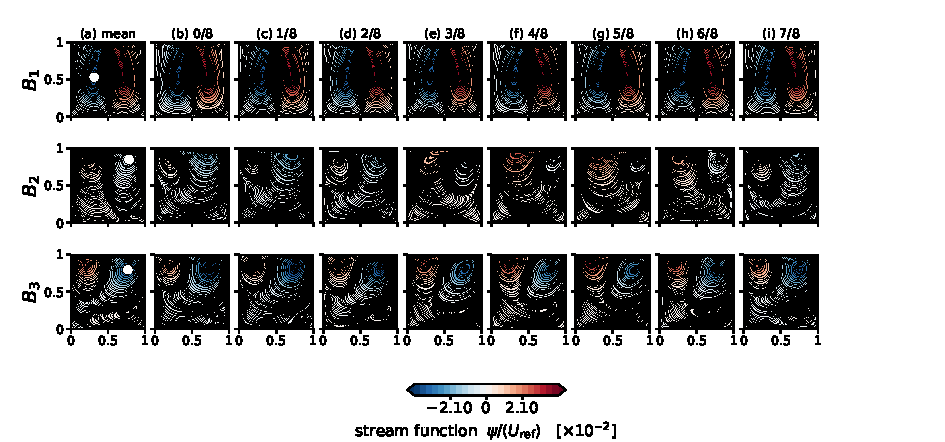
\includegraphics[width=\textwidth]{figS5_branch_topology_phases.pdf}
\caption{All eight phase bins of the three captures of Main Figs.~6--8, on the
same common stream-function scale and contour levels as the main figure. Column (a) is the
time mean, columns (b)--(i) the phase averages at
\(t/T=0,\ 1/8,\dots,7/8\). The phase averages of the first and second halves of
the sampling window differ by at most \(1.0\times10^{-3}\) in relative field
norm for the three branches, so the state is periodic and the four phases
selected for the main figure are representative rather than chosen for
appearance. \(B_1\) is stationary to \(2.7\%\) throughout the cycle; \(B_2\)
shows that its instantaneous structure is not a small perturbation of its mean,
the instantaneous stream-function extrema being one to three times the mean
one, while its mean circulation is \(19\) times weaker. Streamlines are tangent
to the instantaneous velocity and are not particle paths.}
\label{fig:branch_topology_phases}
\end{figure}

\begin{figure}[!ht]
\centering
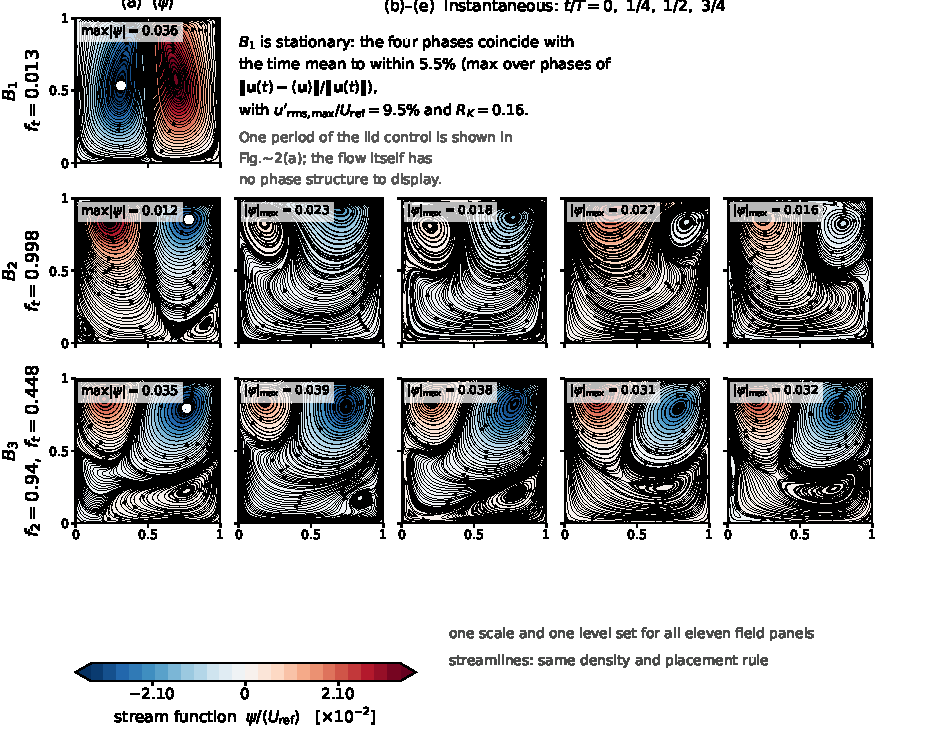
\includegraphics[width=0.85\textwidth]{figS6_branch_topology_panelscale.pdf}
\caption{The layout of Main Fig.~6 with a separate
stream-function scale in every panel, annotated with \(\max|\psi|\) (mean
panels; the instantaneous panels are annotated with their own
\(|\psi|_{\max}\)). The common scale of the main figure is what makes the
\(B_2\) mean cell nearly invisible; this version shows its shape---three
extrema, all within the top tenth of the cavity, with a reversed pair under
the lid---and shows that the \(B_3\) mean circulation is concentrated under the
lid rather than in the mid-depth cells of \(B_1\). The two versions are
complementary and must be read together: only the common scale supports a
quantitative comparison between branches.}
\label{fig:branch_topology_panelscale}
\end{figure}

\subsection{S8.7 Wall-shear estimator and closure uncertainty}
\label{sec:s8_closure}

The identity \(\overline P_{\mathrm{lid}}=\overline D\) of the main text is exact for
the continuous equations, so any residual measured between the two cycle means is a
property of the discrete estimators, not of the physics. Three choices enter the
estimate of \(P_{\mathrm{lid}}\): the velocity used at the wall node, the order of the
one-sided wall-normal derivative, and the number of phases used to average the
product \(U_{\mathrm{lid}}\tau_w\).

\emph{Wall velocity.} The transfer imposes \(U_{\mathrm{lid}}\) through the Zou--He
condition, and the velocity actually recovered at the wall node differs from the
prescribed value by the discrete slip of the scheme. Using the recovered velocity
\(u_x(N-1,\cdot)\) in the product, rather than the prescribed \(U_{\mathrm{lid}}\),
removes most of the residual. With a first-order one-sided derivative the cycle-mean
residual \(\overline P_{\mathrm{lid}}/\overline D-1\) is \(-2.89\%\), \(-0.08\%\) and
\(-0.87\%\) for \(B_1\), \(B_2\) and \(B_3\) when the recovered velocity is used,
against \(+5.30\%\), \(+55.40\%\) and \(+43.56\%\) when the prescribed profile is used.
The prescribed-velocity estimate is therefore discarded: it measures the slip of the
boundary condition, not the power transmitted by the wall. All main-text values use
the recovered velocity.

\emph{Derivative order.} Replacing the first-order one-sided derivative by the
three-point second-order form
\((3u_{N-1}-4u_{N-2}+u_{N-3})/(2\Delta x)\) moves the mean-field residual of \(B_1\)
from \(-2.87\%\) to \(+0.58\%\), i.e.\ it crosses zero, which shows that the
truncation error of the first-order estimate is of the order of the residual itself.
For the cycle means the same change gives \(+1.36\%\) for \(B_1\), but \(+21.5\%\)
for \(B_2\) and \(+16.6\%\) for \(B_3\): the three-point stencil amplifies
lattice-scale noise in the thin Stokes layer of the strongly oscillating lids, where
successive wall-normal velocities differ by more than the signal. The second-order
form is therefore better for the smooth quasi-stationary case and worse for the
unsteady ones, and no single choice is optimal for all three branches. The first-order
form is retained for consistency across the table, and the residual is quoted as
measured.

\emph{Phase quadrature.} The eight stored phase fields are sufficient for the
dissipation, which is a quadratic functional of the instantaneous field, but not for
the power, which is a product of two quantities that both vary within a phase bin.
Averaging the recovered-velocity, first-order power over the eight phases gives
\(-0.27\%\), \(-5.39\%\) and \(-4.46\%\) relative to the direct accumulation over
\(4096\) steps for \(B_1\), \(B_2\) and \(B_3\). The direct accumulation is therefore
used for \(\overline P_{\mathrm{lid}}\) in the main text, and the eight-phase value is
not substituted for it.

Taken together, the three checks bound the estimator uncertainty at a few per cent
for the quasi-stationary branch and at roughly ten per cent for the strongly unsteady
ones. This is why the main text presents \(\overline P_{\mathrm{lid}}=\overline D\) as
an energetic verification with an explicit estimator uncertainty, and why the
conclusions rest on differences of a factor of three rather than on the third
significant digit of the budget.

\clearpage
%=============================================================
\section{S9. Symbolic Regression Configuration and LOCO Details}
%=============================================================

\subsection{S9.1 PySR Configuration}

Each fit---the six leave-one-condition-out refits of Sec.~S9.3---used the same
configuration, listed in Table~\ref{tab:s9_pysr_config}.

\begin{table}[h]
\centering
\caption{PySR hyperparameter configuration, identical for every refit.}
\label{tab:s9_pysr_config}
\small
\begin{tabular}{ll}
\toprule
Parameter & Value\\
\midrule
Populations & 20\\
Iterations & 100 per population\\
Binary operators & \(\{+,\,-,\,\times,\,/\}\)\\
Unary operators & \(\{\sin,\cos,\exp,\mathrm{square},\mathrm{sqrt}\}\)\\
Loss & \(L2\) distance\\
Parsimony coefficient & 0.01\\
Maximum expression size (nodes) & 30\\
Model selection & Best accuracy on the Pareto frontier\\
Random seed & 42, deterministic, serial parallelism\\
Backend & Julia with SymbolicRegression.jl\\
\bottomrule
\end{tabular}
\end{table}

The search is run on standardized inputs and targets, and each returned expression is
converted back to the physical variables \(x\) and \(Re\) before it is evaluated, so that
the constants quoted in Sec.~S9.3 apply directly to \((x,Re)\) without rescaling.

\subsection{S9.2 Input-Output Specification}

The input dataset consists of \(1\,200\) \((x,Re)\) sample pairs, i.e.\ a
\(200\)-point uniform grid on \(x\in[0,1]\) at each of
\(Re\in\{100,300,500,700,900,1000\}\), restricted to \(B_1\)-classified realizations
from the broad campaign. The intermediate
Reynolds values \(Re\in\{400,600,800\}\) are not populated
by any \(B_1\) realization in the campaign and are therefore excluded from the
cross-validation. The target output is the branch-representative stationary
control profile, taken as the time average of
\(U_{\mathrm{lid}}(x,t;Re)\) over the sampling window \(t\in[0,2]\) on
\(64\) time samples, extracted at a fixed actuation energy \(E^\ast=2.0\); among the sampled energy slices,
\(E^\ast=2.0\) is the only one that populates all six Reynolds conditions with
\(B_1\) realizations. The time-averaged profile is used because the \(B_1\)
branch is dominated by the \(n=0\) (stationary) mode, so the time mean fully
characterizes the leading spatial structure while suppressing residual
temporal content. At each condition the representative (largest \(f_2\))
realization is used; the representatives are the seeds listed in
Table~\ref{tab:s5_loco_metrics}.

The regressed quantity is the \emph{peak-normalized} profile,
\(\bar U_{\mathrm{lid}}(x;Re)/\max_x|\bar U_{\mathrm{lid}}(x;Re)|\), so the expression
returned by a fit is a shape and carries no amplitude. The dimensional profile is
recovered by multiplying by the peak scale of the corresponding condition, listed in
Table~\ref{tab:s5_loco_metrics}. Because the target is a time mean, no time variable
appears in any of the returned expressions.

\subsection{S9.3 LOCO Validation Results}

PySR is a stochastic symbolic search: each refit returns the best expression of its own
run, and the six refits are therefore six different expressions rather than six
evaluations of one formula. Tables~\ref{tab:s5_loco_metrics}
and~\ref{tab:s5_loco_expr} report, for each fold, the metrics of the expression that the
fit returned and that expression exactly as recorded.

\begin{table}[h]
\centering
\caption{Per-fold metrics of the recorded \(E^\ast=2.0\) LOCO fits. \(R^2\) and the
root-mean-square error (RMSE) refer to the held-out peak-normalized profile on its
\(200\)-point grid. ``Peak scale'' is \(\max_x|\bar U_{\mathrm{lid}}|\) of the data
profile, which converts an expression into the dimensional mean profile.
\(E_r(\cdot)=\int_0^1(\cdot)^2\,dx\) of that dimensional profile, evaluated for the data
and for the fold expression, and their relative difference, are the amplitude error left
by the description.}
\label{tab:s5_loco_metrics}
\small
\begin{tabular}{ccccccccc}
\toprule
Held-out \(Re\) & Seed & \(f_2\) & \(R^2\) & RMSE & Peak scale & \(E_r^{\mathrm{data}}\) & \(E_r^{\mathrm{SR}}\) & \(\Delta E_r\)\\
\midrule
100  & 3  & 0.884 & 0.8238 & 0.252 & 2.269 & 1.872 & 1.562 & \(-16.6\%\)\\
300  & 2  & 0.738 & 0.8984 & 0.196 & 2.174 & 1.811 & 2.001 & \(+10.5\%\)\\
500  & 2  & 0.866 & 0.9718 & 0.113 & 2.045 & 1.918 & 1.686 & \(-12.1\%\)\\
700  & 13 & 0.943 & 0.9125 & 0.202 & 2.002 & 1.880 & 1.661 & \(-11.7\%\)\\
900  & 1  & 0.739 & 0.9283 & 0.177 & 1.923 & 1.620 & 1.452 & \(-10.4\%\)\\
1000 & 1  & 0.936 & 0.9518 & 0.143 & 2.148 & 1.967 & 2.093 & \(+6.4\%\)\\
\bottomrule
\end{tabular}
\end{table}

\begin{table}[h]
\centering
\caption{The six fold expressions of the \(E^\ast=2.0\) LOCO, recorded exactly as
returned after conversion to \((x,Re)\). In this monospace notation \texttt{*} is
multiplication and \texttt{**} is exponentiation; \texttt{x} and \texttt{Re} are the only
variables. The expression held out at \(Re=500\), the best-scoring fold, contains no
\(Re\) at all, which is the clearest indication that these are per-condition
descriptions rather than one control law.}
\label{tab:s5_loco_expr}
\footnotesize
\begin{tabular}{cp{0.76\textwidth}}
\toprule
Held-out \(Re\) & Expression\\
\midrule
100 & \texttt{\seqsplit{-0.656531744300912*sin(0.000443030877554443*Re + 8.35334751283491*x - 4.78611502315448) - 0.656531744300912*sin(0.000294144339569321*Re + 2.60149100747748*x - (0.00390434404721515*Re - 2.6549539521063)**2*(0.259675841445626*x - 0.129837920722813) - 1.50076365464588) + 0.0835326911204075}}\\
300 & \texttt{\seqsplit{0.0355674592281737 - 0.94948430325695*sin(4.33312505481874*x + sin(3.44682419263376*x + 0.24729648*sin(5.87977914011404*exp(sin(0.003125*Re - 2.0))) - 1.91762330631688) - 2.25663605340937)}}\\
500 & \texttt{\seqsplit{0.038002190814428 - 0.927540972495295*sin(3.4455988*sin(2.27531862008866*x - 1.20059356004433))}}\\
700 & \texttt{\seqsplit{(-0.640381176720972*(1.62396632386904*x - 0.948239180502976)*(3.44682419263376*x - 1.72341209631688) + 1.1369819864629)*sin(-6.24748466244156*x + 0.4038995*cos(-0.00290619096859548*Re + 1.4645397440588*x + 0.895197070384071) + 3.12374233122078) + 0.0421374749638329}}\\
900 & \texttt{\seqsplit{-1.40941323554341*x + 0.645040218519208*sin(-8.63782139306147*x + 0.4854202*sin(0.0032009219983224*Re - 1.23114080131396*x + 0.886964461529331)**2 + 4.31891069653074) + 0.749507753884623}}\\
1000 & \texttt{\seqsplit{-1.39188046572375*x + 0.646718514892542*sin((0.000399479481056593*Re - 2.7101076405283)*(3.44682419263376*x - 1.72341209631688) + 0.31353217) + 0.783949939083173}}\\
\bottomrule
\end{tabular}
\end{table}

The LOCO \(R^2\) ranges from \(0.8238\) at the lowest Reynolds number
(\(Re=100\)) to \(0.9718\) at \(Re=500\), with a mean of \(0.914\). The
\(Re=100\) fold is the most demanding extrapolation case: it lies at the
low-\(Re\) edge of the campaign, so that only the higher side (\(Re=300\)) is
available for interpolation. Three of the six fits
(\(Re=300,700,1000\)) return the same nested argument \(3.4468\,x-1.7234\), whose
phase shift is exactly half a wavelength and which is therefore antisymmetric about the
cavity centre; this recurrence, not a shared closed form, is the reproducible structural
content of the symbolic analysis. The amplitude is not reproduced: the energy of the
dimensional profile rebuilt from a fold expression differs from that of the data profile
by \(-16.6\%\) to \(+10.5\%\), consistent with the fact that the regression target is a
normalized shape. The result therefore shows that the \(B_1\) control family is
described, fold by fold, by compact expressions across the six conditions at which it
is reliably recovered, while the reduced fidelity at the low-\(Re\) edge is
consistent with the weakening \(B_1/B_2\) separation reported in the main text.
The coherence is, moreover, energy-dependent: repeating the LOCO on the
\(E^\ast=0.5\) and \(E^\ast=1.0\) slices yields high scores at most folds but
extrapolation failures at the corresponding edge conditions (\(Re=100\) for
\(E^\ast=0.5\), and \(Re=700\) and \(Re=1000\) for \(E^\ast=1.0\)). The
\(E^\ast=2.0\) slice is thus the only one yielding a uniformly positive LOCO, and
is the one reported in Tables~\ref{tab:s5_loco_metrics}
and~\ref{tab:s5_loco_expr} and in Sec.~S9.3.

%=============================================================
\section{S10. Reproducibility and Computational Pipeline}
%=============================================================

\subsection{S10.1 Software Environment}

Table~\ref{tab:s10_software} lists the software environment used for all the
computations reported here and in the main text.

\begin{table}[h]
\centering
\caption{Software environment for all numerical computations.}
\label{tab:s10_software}
\small
\begin{tabular}{ll}
\toprule
Component & Version\\
\midrule
Python & 3.10.12\\
PyTorch & 2.0.1+cu118\\
NumPy & 1.24.3\\
SciPy & 1.11.1\\
PySR & 0.16.3\\
Julia & 1.9.2\\
GCC (for LBM solver) & 11.4.0\\
OpenMP & 4.5\\
\bottomrule
\end{tabular}
\end{table}

\subsection{S10.2 Hardware}

PINN training was performed on a single NVIDIA A100 GPU (80\,GB HBM2e) with
double-precision computation enabled. The custom C++/OpenMP MRT-LBM solver was
executed on a multi-core CPU workstation (8 cores, 32\,GB RAM) with OpenMP thread
parallelization over lattice rows.

\subsection{S10.3 Computational Cost}

Typical wall-clock times for the main computational components are:
\begin{itemize}
\item One PINN realization (300 pre-training + 3\,000 joint epochs): approximately
  45 minutes on a single A100 GPU.
\item LBM simulation to steady state at \(N=512\): approximately 2 hours on 8 CPU cores.
\item Full 185-realization broad campaign: approximately \(185\times45\approx139\)
  GPU-hours (parallelized across 4 GPUs: approximately 35 hours wall time).
\item \(\lambda_{\mathrm{var}}\) campaign (90 realizations): approximately 68 GPU-hours.
\end{itemize}

\subsection{S10.4 Random Seed Control}

Each realization is assigned a unique integer seed \(s\in\{0,1,\ldots,N_s-1\}\).
At the beginning of each realization the seed is passed to the pseudorandom
generators of the deep-learning framework, of the array library and of the
standard random module, and, for multi-GPU runs, to the device generators as
well. Each realization is therefore strictly reproducible from its seed number.

\subsection{S10.5 Inventory of Numerical Experiments}

Table~\ref{tab:s22_inventory} lists every numerical campaign reported in the main
text and in this document, with the method used and the number of runs. The purpose
is to make the campaign structure auditable: the run counts are stated per study and
are not summed, because the branch-capture representatives reappear among the
iso-energetic transfers, and because the capacity, truncation and aspect-ratio
studies re-run the reference protocol with a single factor changed.

\begin{table}[h]
\centering
\caption{Inventory of the numerical experiments reported in this article. Runs are
counted per campaign. Several studies re-use the same trained control, the same
seeds or the same lattice fields, so the column is not additive and no deduplicated
grand total is claimed.}
\label{tab:s22_inventory}
\small
\begin{tabular}{@{}>{\raggedright\arraybackslash}p{4.3cm} l r >{\raggedright\arraybackslash}p{4.9cm}@{}}
\toprule
Campaign & Method & Runs & Reported in\\
\midrule
Broad \((Re,E^*)\) campaign & PINN & 185 & Main Sec.~3.2; Table~\ref{tab:s1_broad_map}\\
Variance-regularization sweep & PINN & 90 & Sec.~S4; Tables~\ref{tab:s4_wilson} and~\ref{tab:bfirst_ablation}\\
Ten-seed multiplicity & PINN & 10 & Table~\ref{tab:s2_ten_seeds}\\
Network capacity & PINN & 3 & Table~\ref{tab:s6_capacity}\\
Control truncation & PINN & 6 & Table~\ref{tab:s6_truncation}\\
Cavity aspect ratio & PINN & 3 & Table~\ref{tab:s7_aspect_ratio}\\
Fourier vs.\ modified Chebyshev & PINN & 6 & Sec.~S7.2\\
Stationary iso-energetic & LBM-MRT & 12 & Main Sec.~5.1; Table~\ref{tab:s5_isoenergetic}\\
Corner-taper control & LBM-MRT & 3 & Table~\ref{tab:s5_corner}\\
Temporal cycle mean & LBM-MRT & 6 & Table~\ref{tab:s5_temporal}\\
Branch capture & LBM-MRT & 3 & Main Secs.~6.3--6.4; Main Table~4\\
Branch iso-energetic transfers & LBM-MRT & 4 & Table~\ref{tab:branch_isoenergetic}\\
LOCO symbolic refits & PySR & 6 & Tables~\ref{tab:s5_loco_metrics} and~\ref{tab:s5_loco_expr}\\
Classification sensitivity & reanalysis & 0 & Table~\ref{tab:s3_threshold}\\
Dissipation-ratio GCI & derived & 0 & Table~\ref{tab:s5_ratio_gci}\\
\bottomrule
\end{tabular}
\end{table}

The two zero-run rows are re-analyses of runs already listed: the classification
sensitivity relabels the 185 broad-campaign outcomes, and the ratio GCI is formed
from the dissipation values of the iso-energetic campaign. The stationary
iso-energetic row counts four controls on three grids; the corner-taper row adds a
fifth profile on the same three grids. The LOCO row counts symbolic fits, not
simulations.

\subsection{S10.6 Data Availability}

The cell-aggregated record of all 185 runs---realization counts, branch frequencies,
modal statistics and energy calibration per cell---is reported in
Supplementary Table~\ref{tab:s1_broad_map}; the seed-level records retained for the
multiplicity and ablation studies are reported in
Tables~\ref{tab:s2_ten_seeds} and~\ref{tab:s3_ablation}. Further details are
available from the authors upon reasonable request.

\end{document}
